              
                %% bare_jrnl.tex
%% V1.4b
%% 2015/08/26
%% by Michael Shell
%% see http://www.michaelshell.org/
%% for current contact information.
%%
%% This is a skeleton file demonstrating the use of IEEEtran.cls
%% (requires IEEEtran.cls version 1.8b or later) with an IEEE
%% journal paper.
%%
%% Support sites:
%% http://www.michaelshell.org/tex/ieeetran/
%% http://www.ctan.org/pkg/ieeetran
%% and
%% http://www.ieee.org/

%%*************************************************************************
%% Legal Notice:
%% This code is offered as-is without any warranty either expressed or
%% implied; without even the implied warranty of MERCHANTABILITY or
%% FITNESS FOR A PARTICULAR PURPOSE! 
%% User assumes all risk.
%% In no event shall the IEEE or any contributor to this code be liable for
%% any damages or losses, including, but not limited to, incidental,
%% consequential, or any other damages, resulting from the use or misuse
%% of any information contained here.
%%
%% All comments are the opinions of their respective authors and are not
%% necessarily endorsed by the IEEE.
%%
%% This work is distributed under the LaTeX Project Public License (LPPL)
%% ( http://www.latex-project.org/ ) version 1.3, and may be freely used,
%% distributed and modified. A copy of the LPPL, version 1.3, is included
%% in the base LaTeX documentation of all distributions of LaTeX released
%% 2003/12/01 or later.
%% Retain all contribution notices and credits.
%% ** Modified files should be clearly indicated as such, including  **
%% ** renaming them and changing author support contact information. **
%%*************************************************************************


% *** Authors should verify (and, if needed, correct) their LaTeX system  ***
% *** with the testflow diagnostic prior to trusting their LaTeX platform ***
% *** with production work. The IEEE's font choices and paper sizes can   ***
% *** trigger bugs that do not appear when using other class files.       ***                          ***
% The testflow support page is at:
% http://www.michaelshell.org/tex/testflow/


% Please refer to your journal's instructions for other
% options that should be set.
\documentclass[journal,onecolumn]{IEEEtran}
\makeatletter
\long\def\@makecaption#1#2{\ifx\@captype\@IEEEtablestring%
\footnotesize\begin{center}{\normalfont\footnotesize #1}\\
{\normalfont\footnotesize\scshape #2}\end{center}%
\@IEEEtablecaptionsepspace
\else
\@IEEEfigurecaptionsepspace
\setbox\@tempboxa\hbox{\normalfont\footnotesize {#1.}~~ #2}%
\ifdim \wd\@tempboxa >\hsize%
\setbox\@tempboxa\hbox{\normalfont\footnotesize {#1.}~~ }%
\parbox[t]{\hsize}{\normalfont\footnotesize \noindent\unhbox\@tempboxa#2}%
\else
\hbox to\hsize{\normalfont\footnotesize\hfil\box\@tempboxa\hfil}\fi\fi}
\makeatother
%conference
% If IEEEtran.cls has not been installed into the LaTeX system files,
% manually specify the path to it like:
% \documentclass[journal]{../sty/IEEEtran}





% Some very useful LaTeX packages include:
% (uncomment the ones you want to load)


% *** MISC UTILITY PACKAGES ***
%
%\usepackage{ifpdf}
% Heiko Oberdiek's ifpdf.sty is very useful if you need conditional
% compilation based on whether the output is pdf or dvi.
% usage:
% \ifpdf
%   % pdf code
% \else
%   % dvi code
% \fi
% The latest version of ifpdf.sty can be obtained from:
% http://www.ctan.org/pkg/ifpdf
% Also, note that IEEEtran.cls V1.7 and later provides a builtin
% \ifCLASSINFOpdf conditional that works the same way.
% When switching from latex to pdflatex and vice-versa, the compiler may
% have to be run twice to clear warning/error messages.






% *** CITATION PACKAGES ***
%
\usepackage{cite}
% cite.sty was written by Donald Arseneau
% V1.6 and later of IEEEtran pre-defines the format of the cite.sty package
% \cite{} output to follow that of the IEEE. Loading the cite package will
% result in citation numbers being automatically sorted and properly
% "compressed/ranged". e.g., [1], [9], [2], [7], [5], [6] without using
% cite.sty will become [1], [2], [5]--[7], [9] using cite.sty. cite.sty's
% \cite will automatically add leading space, if needed. Use cite.sty's
% noadjust option (cite.sty V3.8 and later) if you want to turn this off
% such as if a citation ever needs to be enclosed in parenthesis.
% cite.sty is already installed on most LaTeX systems. Be sure and use
% version 5.0 (2009-03-20) and later if using hyperref.sty.
% The latest version can be obtained at:
% http://www.ctan.org/pkg/cite
% The documentation is contained in the cite.sty file itself.






% *** GRAPHICS RELATED PACKAGES ***
%
\ifCLASSINFOpdf
  \usepackage[pdftex]{graphicx}
  % declare the path(s) where your graphic files are
  \graphicspath{{./images/}}
  % and their extensions so you won't have to specify these with
  % every instance of \includegraphics
  \DeclareGraphicsExtensions{.pdf,.jpeg,.png}
\else
  % or other class option (dvipsone, dvipdf, if not using dvips). graphicx
  % will default to the driver specified in the system graphics.cfg if no
  % driver is specified.
  \usepackage[dvips]{graphicx}
  % declare the path(s) where your graphic files are
  \graphicspath{./images/}
  % and their extensions so you won't have to specify these with
  % every instance of \includegraphics
  \DeclareGraphicsExtensions{.eps}
\fi
% graphicx was written by David Carlisle and Sebastian Rahtz. It is
% required if you want graphics, photos, etc. graphicx.sty is already
% installed on most LaTeX systems. The latest version and documentation
% can be obtained at: 
% http://www.ctan.org/pkg/graphicx
% Another good source of documentation is "Using Imported Graphics in
% LaTeX2e" by Keith Reckdahl which can be found at:
% http://www.ctan.org/pkg/epslatex
%
% latex, and pdflatex in dvi mode, support graphics in encapsulated
% postscript (.eps) format. pdflatex in pdf mode supports graphics
% in .pdf, .jpeg, .png and .mps (metapost) formats. Users should ensure
% that all non-photo figures use a vector format (.eps, .pdf, .mps) and
% not a bitmapped formats (.jpeg, .png). The IEEE frowns on bitmapped formats
% which can result in "jaggedy"/blurry rendering of lines and letters as
% well as large increases in file sizes.
%
% You can find documentation about the pdfTeX application at:
% http://www.tug.org/applications/pdftex
\usepackage[caption=false, font=footnotesize]{subfig}




% *** MATH PACKAGES ***
%
%\usepackage{amsmath}
% A popular package from the American Mathematical Society that provides
% many useful and powerful commands for dealing with mathematics.
%
% Note that the amsmath package sets \interdisplaylinepenalty to 10000
% thus preventing page breaks from occurring within multiline equations. Use:
%\interdisplaylinepenalty=2500
% after loading amsmath to restore such page breaks as IEEEtran.cls normally
% does. amsmath.sty is already installed on most LaTeX systems. The latest
% version and documentation can be obtained at:
% http://www.ctan.org/pkg/amsmath





% *** SPECIALIZED LIST PACKAGES ***
%
%\usepackage{algorithmic}
% algorithmic.sty was written by Peter Williams and Rogerio Brito.
% This package provides an algorithmic environment fo describing algorithms.
% You can use the algorithmic environment in-text or within a figure
% environment to provide for a floating algorithm. Do NOT use the algorithm
% floating environment provided by algorithm.sty (by the same authors) or
% algorithm2e.sty (by Christophe Fiorio) as the IEEE does not use dedicated
% algorithm float types and packages that provide these will not provide
% correct IEEE style captions. The latest version and documentation of
% algorithmic.sty can be obtained at:
% http://www.ctan.org/pkg/algorithms
% Also of interest may be the (relatively newer and more customizable)
% algorithmicx.sty package by Szasz Janos:
% http://www.ctan.org/pkg/algorithmicx



% *** ALIGNMENT PACKAGES ***
%
%\usepackage{array}
% Frank Mittelbach's and David Carlisle's array.sty patches and improves
% the standard LaTeX2e array and tabular environments to provide better
% appearance and additional user controls. As the default LaTeX2e table
% generation code is lacking to the point of almost being broken with
% respect to the quality of the end results, all users are strongly
% advised to use an enhanced (at the very least that provided by array.sty)
% set of table tools. array.sty is already installed on most systems. The
% latest version and documentation can be obtained at:
% http://www.ctan.org/pkg/array


% IEEEtran contains the IEEEeqnarray family of commands that can be used to
% generate multiline equations as well as matrices, tables, etc., of high
% quality.




% *** SUBFIGURE PACKAGES ***
%\ifCLASSOPTIONcompsoc
%  \usepackage[caption=false,font=normalsize,labelfont=sf,textfont=sf]{subfig}
%\else
%  \usepackage[caption=false,font=footnotesize]{subfig}
%\fi
% subfig.sty, written by Steven Douglas Cochran, is the modern replacement
% for subfigure.sty, the latter of which is no longer maintained and is
% incompatible with some LaTeX packages including fixltx2e. However,
% subfig.sty requires and automatically loads Axel Sommerfeldt's caption.sty
% which will override IEEEtran.cls' handling of captions and this will result
% in non-IEEE style figure/table captions. To prevent this problem, be sure
% and invoke subfig.sty's "caption=false" package option (available since
% subfig.sty version 1.3, 2005/06/28) as this is will preserve IEEEtran.cls
% handling of captions.
% Note that the Computer Society format requires a larger sans serif font
% than the serif footnote size font used in traditional IEEE formatting
% and thus the need to invoke different subfig.sty package options depending
% on whether compsoc mode has been enabled.
%
% The latest version and documentation of subfig.sty can be obtained at:
% http://www.ctan.org/pkg/subfig




% *** FLOAT PACKAGES ***
%
%\usepackage{fixltx2e}
% fixltx2e, the successor to the earlier fix2col.sty, was written by
% Frank Mittelbach and David Carlisle. This package corrects a few problems
% in the LaTeX2e kernel, the most notable of which is that in current
% LaTeX2e releases, the ordering of single and double column floats is not
% guaranteed to be preserved. Thus, an unpatched LaTeX2e can allow a
% single column figure to be placed prior to an earlier double column
% figure.
% Be aware that LaTeX2e kernels dated 2015 and later have fixltx2e.sty's
% corrections already built into the system in which case a warning will
% be issued if an attempt is made to load fixltx2e.sty as it is no longer
% needed.
% The latest version and documentation can be found at:
% http://www.ctan.org/pkg/fixltx2e


%\usepackage{stfloats}
% stfloats.sty was written by Sigitas Tolusis. This package gives LaTeX2e
% the ability to do double column floats at the bottom of the page as well
% as the top. (e.g., "\begin{figure*}[!b]" is not normally possible in
% LaTeX2e). It also provides a command:
%\fnbelowfloat
% to enable the placement of footnotes below bottom floats (the standard
% LaTeX2e kernel puts them above bottom floats). This is an invasive package
% which rewrites many portions of the LaTeX2e float routines. It may not work
% with other packages that modify the LaTeX2e float routines. The latest
% version and documentation can be obtained at:
% http://www.ctan.org/pkg/stfloats
% Do not use the stfloats baselinefloat ability as the IEEE does not allow
% \baselineskip to stretch. Authors submitting work to the IEEE should note
% that the IEEE rarely uses double column equations and that authors should try
% to avoid such use. Do not be tempted to use the cuted.sty or midfloat.sty
% packages (also by Sigitas Tolusis) as the IEEE does not format its papers in
% such ways.
% Do not attempt to use stfloats with fixltx2e as they are incompatible.
% Instead, use Morten Hogholm'a dblfloatfix which combines the features
% of both fixltx2e and stfloats:
%
% \usepackage{dblfloatfix}
% The latest version can be found at:
% http://www.ctan.org/pkg/dblfloatfix




%\ifCLASSOPTIONcaptionsoff
%  \usepackage[nomarkers]{endfloat}
% \let\MYoriglatexcaption\caption
% \renewcommand{\caption}[2][\relax]{\MYoriglatexcaption[#2]{#2}}
%\fi
% endfloat.sty was written by James Darrell McCauley, Jeff Goldberg and 
% Axel Sommerfeldt. This package may be useful when used in conjunction with 
% IEEEtran.cls'  captionsoff option. Some IEEE journals/societies require that
% submissions have lists of figures/tables at the end of the paper and that
% figures/tables without any captions are placed on a page by themselves at
% the end of the document. If needed, the draftcls IEEEtran class option or
% \CLASSINPUTbaselinestretch interface can be used to increase the line
% spacing as well. Be sure and use the nomarkers option of endfloat to
% prevent endfloat from "marking" where the figures would have been placed
% in the text. The two hack lines of code above are a slight modification of
% that suggested by in the endfloat docs (section 8.4.1) to ensure that
% the full captions always appear in the list of figures/tables - even if
% the user used the short optional argument of \caption[]{}.
% IEEE papers do not typically make use of \caption[]'s optional argument,
% so this should not be an issue. A similar trick can be used to disable
% captions of packages such as subfig.sty that lack options to turn off
% the subcaptions:
% For subfig.sty:
% \let\MYorigsubfloat\subfloat
% \renewcommand{\subfloat}[2][\relax]{\MYorigsubfloat[]{#2}}
% However, the above trick will not work if both optional arguments of
% the \subfloat command are used. Furthermore, there needs to be a
% description of each subfigure *somewhere* and endfloat does not add
% subfigure captions to its list of figures. Thus, the best approach is to
% avoid the use of subfigure captions (many IEEE journals avoid them anyway)
% and instead reference/explain all the subfigures within the main caption.
% The latest version of endfloat.sty and its documentation can obtained at:
% http://www.ctan.org/pkg/endfloat
%
% The IEEEtran \ifCLASSOPTIONcaptionsoff conditional can also be used
% later in the document, say, to conditionally put the References on a 
% page by themselves.
% \usepackage{caption}



% *** PDF, URL AND HYPERLINK PACKAGES ***
%
\usepackage{url}
% url.sty was written by Donald Arseneau. It provides better support for
% handling and breaking URLs. url.sty is already installed on most LaTeX
% systems. The latest version and documentation can be obtained at:
% http://www.ctan.org/pkg/url
% Basically, \url{my_url_here}.




% *** Do not adjust lengths that control margins, column widths, etc. ***
% *** Do not use packages that alter fonts (such as pslatex).         ***
% There should be no need to do such things with IEEEtran.cls V1.6 and later.
% (Unless specifically asked to do so by the journal or conference you plan
% to submit to, of course. )


% correct bad hyphenation here
% \hyphenation{op-tical net-works semi-conduc-tor}

\usepackage{listings}

\usepackage{xcolor}
\definecolor{codegreen}{rgb}{0,0.6,0}
\definecolor{codegray}{rgb}{0.5,0.5,0.5}
\definecolor{codepurple}{rgb}{0.58,0,0.82}
\definecolor{backcolour}{rgb}{0.95,0.95,0.92}


\newcommand{\code}[1]{\texttt{#1}}
%Code listing style named "mystyle"
\lstdefinestyle{mystyle}{
  backgroundcolor=\color{backcolour}, commentstyle=\color{codegreen},
  keywordstyle=\color{magenta},
  numberstyle=\tiny\color{codegray},
  stringstyle=\color{codepurple},
  basicstyle=\ttfamily\footnotesize,
  breakatwhitespace=false,         
  breaklines=true,                 
  captionpos=b,                    
  keepspaces=true,                 
  numbers=left,                    
  numbersep=5pt,                  
  showspaces=false,                
  showstringspaces=false,
  showtabs=false,                  
  tabsize=2
}
\lstset{style=mystyle}

% \usepackage{graphicx}
%\graphicspath{ {./images/} }

\begin{document}
%
% paper title
% Titles are generally capitalized except for words such as a, an, and, as,
% at, but, by, for, in, nor, of, on, or, the, to and up, which are usually
% not capitalized unless they are the first or last word of the title.
% Linebreaks \\ can be used within to get better formatting as desired.
% Do not put math or special symbols in the title.
\title{Container~in~Depth: A Comprehensive\\Approach to Resolving\\Linux Packaging and Dependency Issues }
%
%
% author names and IEEE memberships
% note positions of commas and nonbreaking spaces ( ~ ) LaTeX will not break
% a structure at a ~ so this keeps an author's name from being broken across
% two lines.
% use \thanks{} to gain access to the first footnote area
% a separate \thanks must be used for each paragraph as LaTeX2e's \thanks
% was not built to handle multiple paragraphs
%

\author{Simon~Zam,~\IEEEmembership{24256816, Author, ~Auckland~University~of~Technology,}\\
        Dr.~Jian~Yu,~\IEEEmembership{Supervisor, ~Associate~Professor, ~Auckland University~of~Technology}% <-this % stops a space
        }

% note the % following the last \IEEEmembership and also \thanks - 
% these prevent an unwanted space from occurring between the last author name
% and the end of the author line. i.e., if you had this:
% 
% \author{....lastname \thanks{...} \thanks{...} }
%                     ^------------^------------^----Do not want these spaces!
%
% a space would be appended to the last name and could cause every name on that
% line to be shifted left slightly. This is one of those "LaTeX things". For
% instance, "\textbf{A} \textbf{B}" will typeset as "A B" not "AB". To get
% "AB" then you have to do: "\textbf{A}\textbf{B}"
% \thanks is no different in this regard, so shield the last } of each \thanks
% that ends a line with a % and do not let a space in before the next \thanks.
% Spaces after \IEEEmembership other than the last one are OK (and needed) as
% you are supposed to have spaces between the names. For what it is worth,
% this is a minor point as most people would not even notice if the said evil
% space somehow managed to creep in.



% The paper headers
%\markboth{Journal of \LaTeX\ Class Files,~Vol.~14, No.~8, August~2015}%
%{Shell \MakeLowercase{\textit{et al.}}: Bare Demo of IEEEtran.cls for IEEE Journals}
% The only time the second header will appear is for the odd numbered pages
% after the title page when using the twoside option.
% 
% *** Note that you probably will NOT want to include the author's ***
% *** name in the headers of peer review papers.                   ***
% You can use \ifCLASSOPTIONpeerreview for conditional compilation here if
% you desire.




% If you want to put a publisher's ID mark on the page you can do it like
% this:
%\IEEEpubid{0000--0000/00\$00.00~\copyright~2015 IEEE}
% Remember, if you use this you must call \IEEEpubidadjcol in the second
% column for its text to clear the IEEEpubid mark.



% use for special paper notices
%\IEEEspecialpapernotice{(Invited Paper)}




% make the title area
\maketitle

% As a general rule, do not put math, special symbols or citations
% in the abstract or keywords.
\begin{abstract}
Analyse and review the low-level container architecture, finds a solution for various Linux packaging systems, different operating systems with various packaging designs, focus on unifying the branching of Linux packaging system by utilising container environment.

\end{abstract}

% Note that keywords are not normally used for peerreview papers.
\begin{IEEEkeywords}
Linux, Unix, Packaging, Repository, Operating System, Containerisation, Open-source, Dependency, Container, Podman, Docker, Kernel.
\end{IEEEkeywords}






% For peer review papers, you can put extra information on the cover
% page as needed:
% \ifCLASSOPTIONpeerreview
% \begin{center} \bfseries EDICS Category: 3-BBND \end{center}
% \fi
%
% For peerreview papers, this IEEEtran command inserts a page break and
% creates the second title. It will be ignored for other modes.
\IEEEpeerreviewmaketitle



\section{Introduction and Background}
% The very first letter is a 2 line initial drop letter followed
% by the rest of the first word in caps.
% 
% form to use if the first word consists of a single letter:
% \IEEEPARstart{A}{demo} file is ....
% 
% form to use if you need the single drop letter followed by
% normal text (unknown if ever used by the IEEE):
% \IEEEPARstart{A}{}demo file is ....
% 
% Some journals put the first two words in caps:
% \IEEEPARstart{T}{his demo} file is ....
% 
% Here we have the typical use of a "T" for an initial drop letter
% and "HIS" in caps to complete the first word.
\subsection{Introduction}
\IEEEPARstart{L}{inux} dependency hell has been a problem since the dawn of the Linux operating system. Like Unix based Linux, the Windows NT based Windows operating system also has a DLL hell problem. Unlike Windows, which is a closed source and follows a linear development model, Linux's strength lies in its customisability and the freedom it offers to users. However, this flexibility comes at the cost of branching architecture with numerous distributions, ranging from Alpine, Arch, Debian, Slackware, SUSE, Red Hat, Android and many others. Different distributions have different packaging systems with different system designs, and maintaining packages for all the numerous systems has been a problem for software developers. Some distributions even have multiple packaging systems, such as Debian-based systems that use '.deb' packages and are managed by tools such as 'apt' or 'dpkg', while Red Hat-based systems use '.rpm' packages managed by 'yum' or 'dnf'. This diversity in packaging systems becomes a hassle for developers to produce applications to cover all of this. To make matters worse, many new Linux distributions are rolling out every day which use different packaging styles. 

Windows NT partially solved DLL hell problem by Static linking: statically link own DLLs for each application and Portable Packages: applications bundle required DLLs with its own private DLLs. Unlike Windows, Linux operating systems are diverse. Various non-profit organisations and proprietary companies developed different kinds of Linux based operating systems with their own packaging system which becomes incompatible with one another. 

This research paper aims to solve this problem by unionising all the packaging systems into containers which can be run on every Linux operating system with consistency and linearity. The concept of containers present a viable solution where containers are lightweight and portable, encapsulating an application and its dependencies into a single image unit that can run easily across every environment. This is achieved with containerisation technologies like Docker, Podman, LXC, LXD, containerd which leverages Linux kernel features such as namespaces, cgroups and jailing. For future reference, this research prototype is based on Podman. 
% You must have at least 2 lines in the paragraph with the drop letter
% (should never be an issue)

% \hfill mds
 
% \hfill August 26, 2015
\newpage
\subsection{Background and Motivation}
The Linux ecosystem has long been a complex with packaging and dependency management. As a user who used multiple Linux distributions, starting the journey from Debian to various other distributions, the author has experienced the frustrations of dealing with different package managers. Each package manager has their own strengths and weaknesses, handling them in their own ways. While some distributions excel in certain areas such as package availability or update frequently, others usually leave the job of compiling the source code to user for compatibility and openness. E.g. Linux from Scratch, Gentoo, Arch (AUR). 

As an open-source developer, this problem becomes frustrating and tedious. The diversity of Linux distributions becomes a double-edged sword where developers need to take account of all packaging systems, dependency chains, and versioning schemes. Even for standalone binaries, sometimes, the application has to rely on larger libraries. The advent of containerisation, particularly with Docker, has been a game-changer in this space. 

By encapsulating an application and its dependencies within a container, developers can ensure reproducible and reliable application across different environments. The author’s experience with containerisation began with a project where the author needed to deploy an application across multiple different servers. Containers not only simplified the deployment process but were also able to help the application run smoothly on any underlying Linux operating system. This experience sparked an idea that what if containers could be used to deliver all applications not only CLI (Command Line) but also GUI (Graphical User Interface), effectively decoupling them from the underlying distribution package manager? 

The idea of using containers to deliver applications is both exciting and promising. However, there are some hurdles to overcome. As someone who has been solving the complexities of Linux for years, the author is eager to explore this approach and see how it might change the future of application delivery in the Linux ecosystem. 

\newpage
\section{Literature Review}

Eelco Dolstra and Andres Loh\cite{10.1145/1411204.1411255}\cite{10.1145/1411203.1411255} introduced NixOS, a purely functional Linux distribution, offers a distinct paradigm for managing software packages and system configurations. Unlike conventional distributions that manage packages imperatively, NixOS use the Nix package manager to build and manage all software in isolated, cryptographically hashed environments. This approach ensures that every package and its dependencies are uniquely identified and isolated, eliminating "dependency hell" and guaranteeing bit-for-bit reproducibility across different systems. Furthermore, its declarative system configuration allows for atomic upgrades and rollbacks, which makes robust mechanisms for system stability and recovery from failed updates. However, a key distinction from container technologies, which are the focus of this paper, is that NixOS primarily addresses dependency and reproducibility challenges at the system and package build level. It does not inherently provide the same granular runtime process isolation, resource limiting, or lightweight application portability across arbitrary host operating systems that container runtime like Docker or Podman. While Nix can be used to build container images, its native main strength in managing the entire operating system's state, rather than encapsulating individual applications for deployment in diverse, pre-existing host environments.

In "A Study of Application Sandbox Policies in Linux," \cite{10.1145/3532105.3535016} provide the first comprehensive analysis of application sandbox policies within the emerging Flatpak and Snap ecosystems on Linux desktop operating systems. The paper investigates 283 matching applications across both platforms, revealing that Flatpak and Snap significantly enhance Linux platform security, with a high percentage of applications (90.1\% of Snaps and 58.3\% of Flatpaks) contained by tamper-proof sandboxes. While the study finds evidence that package maintainers actively strive for least-privilege policies, often favouring fine-grained permissions, it also highlights the inherent difficulty and error-proneness in defining such policies, evidenced by frequent mismatches and instances of over- or under-privilege between Flatpak and Snap versions of the same application. Although the paper focus on theory to address the packaging security, it does not show the result and prototype to implement in real application.

This paper by Antunes and Vardasca (2014)\cite{ANTUNES2014649} presents a performance analysis between FreeBSD jail environments and traditional virtualisation solutions for cloud computing implementations. The authors conducted tests using SSH, HTTP, and NetBIOS protocols to evaluate resource consumption and data access performance across different cases, including single and concurrent access patterns. Their findings demonstrate that jail environments significantly outperform virtualised solutions, achieving performance improvements of over 50\% while consuming fewer hardware resources which requiring only minimal CPU (~2.5\%), memory (~20MB), and storage (~150MB) compared to virtual machines that demand considerably more resources for both the hypervisor and individual instances. The study shows that jail environments maintain consistent performance regardless of the number of running instances, whereas virtual machines experience performance degradation as additional instances are deployed. However, the authors acknowledge the limitation of jail-based solutions such as the loss of operating system flexibility while all containers must share the same kernel as the host system. Despite the constraint, they conclude that for specific cloud computing scenarios focused on data access and service provision rather than diverse operating system requirements, jail environments offer great alternative that can enhance performance while reducing infrastructure costs

In the paper "OPIUM: Optimal Package Install/Uninstall Manager," Tucker et al.\cite{10.1109/ICSE.2007.59} address the limitations of traditional Linux package managers like apt-get and yum, which rely on heuristics, which cause inability to optimise installations based on user preferences. The authors propose OPIUM, a package management tool that utilise SAT, pseudo-boolean, and Integer Linear Programming solvers to model package dependencies and conflicts as constraint and optimisation problems. OPIUM offers two key advantages, it guarantee a solution if one exists, and it can optimise installations according to user-defined objective functions, such as minimising download size or maximising package popularity. Through an evaluation against Debian's apt-get using 600 real-world installation traces, the authors demonstrate that OPIUM is practically usable despite being slower than apt-get, OPIUM features provide concrete benefits where successfully handling cases where apt-get fails and finding better solutions in terms of packages removed and data downloaded.

Ryding and Johansson (2020), in their study "Jails vs Docker: A performance comparison of different container technologies,"\cite{Ryding_Johansson_2020} conducted a performance evaluation comparing FreeBSD Jails and Docker on Linux. Utilising benchmarking tools for CPU, memory, disk I/O, network, and startup times across varying container counts (1 to 32), they aimed to determine the efficiency and stability of each technology. The findings revealed that Docker generally outperformed Jails in CPU efficiency and disk read performance across most test cases. Notably, Docker demonstrated better utilisation of shared resources and higher stability (lower result variance) when running multiple containers, contradicting some earlier research. Conversely, Jails proved significantly faster in container startup times and showed superior network performance with a low number of containers. The authors concluded that while Docker appears superior for overall performance and stability, Jails remain competitive or better in specific scenarios like startup speed and low-container network performance, also discussing how feature adoption (like Docker's platform independence and repository system) could benefit Jails. A key limitation acknowledged by the authors was the use of the default file-systems (ZFS for FreeBSD and EXT4 for Linux), which may have influenced the disk I/O performance results.

\newpage
\section{Research Questions and Scoping}
\subsection{Research Questions}
We articulate the research questions that directly address the core problem of Linux packaging and dependency management, as introduced in the introduction, and clarify the specific gap identified in the literature review regarding the potential of a comprehensive container-based solution. We also define the scope of this study to establish clear boundaries for the investigation, guiding the methodology and expected outcomes. Based on the identified challenges with traditional Linux packaging and the potential of container technology, this research seeks to answer the following questions:

\begin{itemize}[\IEEEsetlabelwidth{Z}]
    \item[RQ1:] To what extent does a comprehensive containerisation approach, encompassing both command-line and graphical user interface (GUI) applications, effectively mitigate the "dependency hell" problem in Linux compared to traditional packaging methods, and what specific dependency challenges persist within this model?
    \item[RQ2:] What are the key security implications and necessary mitigation strategies when implementing a universal container-based system for managing diverse Linux applications, with a particular focus on the unique security considerations introduced by integrating graphical user interface (GUI) applications within this framework?
    \item[RQ3:] What are the primary design considerations for building a container-based application packaging system for a comprehensive Linux environment (including GUI applications), and how does this approach impact the end-user experience in terms of application installation, execution, and integration? 
\end{itemize}


\subsection{Aim}
The primary aim of this research is to propose and critically evaluate the feasibility and effectiveness of adopting a comprehensive container-based model for resolving Linux application packaging and dependency issues across the entire application spectrum, including GUI applications. Specifically, the study aims to assess the potential of containers to significantly reduce or eliminate dependency conflicts for all types of Linux applications and identify and analyse the security implications inherent in a universal containerised application ecosystem, proposing relevant mitigation strategies, particularly concerning GUI application integration. This research also aim to explore the architectural and design considerations required for such a system and evaluate its potential impact on the end-user experience. 

Through these aims, the research seeks to determine if a comprehensive container strategy is a viable and beneficial paradigm shift for Linux application management. 

\subsection{Scope of the Study}
The scope of this study is defined to provide a focused and achievable investigation into the proposed comprehensive container-based packaging model. 

Included: 
\begin{itemize}[\IEEEsetlabelwidth{Z}]
    \item Analysis of the "dependency hell" problem within traditional Linux packaging (e.g., package managers like APT, YUM/DNF). 
    \item Investigation of how container technology (using Docker and Podman as representative examples) fundamentally addresses dependency isolation. 
    \item Examination of the challenges and potential solutions for containerising diverse application types, with a specific focus on the unique requirements and complexities of graphical user interface (GUI) applications (e.g., display server integration, desktop environment interaction). 
    \item Analysis of the security implications of running a wide range of applications, including GUI apps, within containers, covering aspects like isolation, privilege escalation, and host system interaction. 
    \item Exploration of high-level architectural and design principles for a system that utilises containers as the primary application of packaging and distribution mechanisms. 
    \item Consideration of the end-user experience, including aspects like application discovery, installation, updates, startup times, and integration with the host environment, based on qualitative analysis and conceptual metrics. 
\end{itemize}

Excluded:
\begin{itemize}
    \item In-depth technical analysis of the internal implementation details of specific container runtime or image formats (unless directly relevant to dependency or security mechanisms discussed). 
    \item Detailed performance benchmarking of containerised applications versus native installed applications beyond the scope of perceived user experience (e.g., micro-benchmarks not related to typical application usage). 
    \item Comprehensive comparison with all alternative modern packaging formats (e.g., Snap, Flatpak) – while they may be mentioned in the literature review as related work, the focus is specifically on the universal container model. 
    \item Analysis of enterprise-scale container orchestration platforms (e.g., Kubernetes) – the focus is on the application packaging and execution model for a single-user or desktop environment. 
    \item Development of a fully functional prototype system – the study is primarily analytical and conceptual, though it may draw upon existing tools and experiments. 
    \item Detailed legal or licensing implications of software distribution via containers. 
\end{itemize}

\subsection{Contributions of the study}
This study aims to contribute to the understanding of Linux application management by providing a comprehensive analysis of the potential and challenges of using container technology as a universal packaging and dependency resolution mechanism, specifically addressing the often-overlooked complexities of incorporating GUI applications into such a model. By evaluating its effectiveness against dependency hell, analysing its security landscape, and exploring design and user experience considerations, this research offers valuable insights for future operating system design, application distribution strategies, and the ongoing effort to simplify the Linux desktop experience. It provides a structured framework for evaluating containerisation not just as an isolation tool for servers, but as a fundamental shift in how all applications, including graphical ones, can be delivered and managed on Linux systems.

\newpage
\section{Research Method}
\subsection{Research Plan}
\subsubsection{Foundational Research Phase}

This initial phase involves a comprehensive review of existing literature to: 

\begin{itemize}

    \item Identify and Characterise Current Challenges: Systematically analyse documented issues related to traditional Linux packaging (e.g., DEB, RPM), universal package formats (e.g., Flatpak, Snap, AppImage), and existing dependency management systems. This includes "dependency hell," library version conflicts, platform inconsistencies, and difficulties in application portability. 
    \item Survey Existing Containerisation Solutions: Review the architecture, benefits, and limitations of prevalent containerisation technologies like Docker and Podman, focusing on their current use cases, particularly in server-side deployments. 
    \item Examine Current Approaches to UI Application Containerisation: Investigate existing techniques, tools (e.g., X11 forwarding, Wayland integration, PipeWire for audio/video), and community efforts aimed at running graphical applications within containers. This will highlight current best practices and unresolved challenges. 
    \item Establish a Baseline: Define the current state-of-the-art and identify gaps that the proposed universal containerisation approach aims to address. 
    \item Choose a methodology: We will use systematic review methodology for this paper as it is the most compatible with our research questions and objectives. This methodology is more effective than others and strongly align with our approach.

\end{itemize}

\subsubsection{Proof-of-Concept (PoC) Prototype Development and Implementation Phase}

\begin{itemize}
    \item Selection of Target Applications: A curated set of applications will be chosen to represent various categories: 
    \begin{itemize}
        \item Complex UI applications: e.g., IDEs, web browsers, office suites, multimedia applications. 
        \item Applications with specific hardware dependencies: e.g., applications requiring GPU acceleration, specific device access (e.g., webcam, microphone). 
    \end{itemize}
    \item Containerisation Strategy: 
    \begin{itemize}
        \item Technology Choice: Both Docker and Podman will be utilised to create container images, allowing for a comparison of their suitability for this universal approach. Standard Dockerfiles/Containerfiles will be developed. 
        \item Base Image Selection: Minimal base images (e.g., Alpine Linux, Ubuntu) will be prioritised to reduce overhead, while also considering compatibility with application dependencies. 
        \item UI Integration Techniques: Implementation and testing of various methods for UI rendering and interaction, including:
        \begin{itemize}
            \item X11 socket sharing and forwarding. 
            \item Wayland proxying solutions. 
            \item Integration with host sound systems (e.g., PulseAudio, PipeWire). 
        \end{itemize}
        \item Persistence and Configuration: Strategies for managing user data, application configurations, and ensuring seamless updates will be designed and implemented (e.g., volume mounts, environment variables). 
        \item Security Considerations: Implementation of best practices for container security, including user namespacing, Seccomp profiles, and AppArmor/SELinux where appropriate, to ensure that containerised UI applications do not pose undue security risks. 

    \end{itemize}
\end{itemize}

\subsubsection{Evaluation and Comparative Analysis Phase}

The containerised applications developed in Prototype Development Phase will be rigorously evaluated against several key metrics and compared with traditional installation methods and other universal packaging formats.
\begin{itemize}
    \item Evaluation Metrics:
    \begin{itemize}
        \item Dependency Resolution and Portability:
        \begin{itemize}
            \item Success rate of containerising selected applications.
            \item Ease of deployment across different Linux distributions (e.g., Ubuntu, Fedora, Arch Linux).
            \item Absence of host system library conflicts.
        \end{itemize}
        \item Performance:
        \begin{itemize}
            \item Startup Time: Time taken for the application to launch and become responsive.
            \item Resource Consumption: CPU usage, RAM footprint, and disk space (image size vs. installed size of traditional packages).
            \item Runtime Performance: Responsiveness and perceived smoothness of UI applications, especially those requiring graphics or multimedia capabilities. Standardised benchmarks will be used where applicable (e.g., GPU tasks).
        \end{itemize}
        \item Usability and User Experience (UX):
        \begin{itemize}
            \item Seamlessly integrable with the host desktop environment (e.g., file access, theme consistency, notifications).
            \item Ease of installation, update, and removal for the end-user.
        \end{itemize}
        \item Developer Experience (DX):
        \begin{itemize}
            \item Complexity of creating and maintaining container definitions (Dockerfiles/Containerfiles).
            \item Ease of debugging applications running within containers.
        \end{itemize}
        \item Isolation and Security:
        \begin{itemize}
            \item Effectiveness of process and file-system isolation.
            \item Assessment of the attack surface compared to natively installed applications.
        \end{itemize}
    \end{itemize}
    \item Comparative Baselines:
    \begin{itemize}
        \item Native Packaging: Applications installed via the system package manager (e.g., `apt`, `dnf`).
        \item Other Universal Formats: Comparison with existing Flatpak or Snap versions of different applications, if available and mature.
    \end{itemize}
    \item Data Collection Methods:    
    \begin{itemize}
        \item Benchmarking Tools: Standardised tools for performance measurement (e.g., `time` command, `htop`, `iotop`, custom scripting for UI responsiveness), manual user testing.
        \item System Logs and Monitoring: Collection of system logs and resource usage data during application execution.
        \item Qualitative Assessment: Documented on ease of use and overall user/developer experience. For UI applications.
        \item Reproducibility: All container definitions, test scripts, and methodologies will be documented for reproducibility.
    \end{itemize}
\end{itemize}
\subsubsection{Data Analysis}

The data collected in Evaluation Phase will be analysed as follows:
\begin{itemize}
    \item Quantitative data (performance metrics, resource usage) will be analysed to identify differences between the containerised version and native. Results will be shown using tables, charts, and graphs.
    \item Qualitative data (usability, DX) will be analysed to identify patterns, strengths, and drawbacks of the proposed containerisation approach.
\end{itemize}
\newpage
\subsection{Research Prototype Development}
The prototype will be developed using Podman, developed by RedHat which is Open Container Initiative (OCI)-compliant. Podman is based on the libpod library API, which is identical to Docker and the application images will be based on the Containerfile format.

\subsubsection{Prototype 1(Brave Browser)}
This Prototype was developed for Brave Browser, based on an Ubuntu container image. Brave Browser is based on Chromium and this application is chosen to demonstrate that all chromium based applications are able to run in a container.

\begin{lstlisting}[language=Bash]
FROM ubuntu:latest

RUN apt update && apt install -yq --no-install-recommends \
        ca-certificates \
        gnupg \
        libgl1 \
        libpulse0 \
        curl \
        libegl1-mesa \
    && curl -fsSLo /usr/share/keyrings/brave-browser-archive-keyring.gpg https://brave-browser-apt-release.s3.brave.com/brave-browser-archive-keyring.gpg \
    && echo "deb [signed-by=/usr/share/keyrings/brave-browser-archive-keyring.gpg arch=amd64] https://brave-browser-apt-release.s3.brave.com/ stable main"|tee /etc/apt/sources.list.d/brave-browser-release.list \
    && apt update && apt install -yq --no-install-recommends brave-browser \
    && fc-cache -fv \
    && rm -rf /var/lib/apt/lists/* \
    && apt autoclean && apt autoremove --purge && apt clean \
    && find / -xdev -type f -perm /u+s -exec chmod -c u-s {} \; \
    && find / -xdev -type f -perm /g+s -exec chmod -c g-s {} \; \
    && echo "default-server = unix:/run/user/1000/pulse/native\nautospawn = no\ndaemon-binary = /bin/true\nenable-shm = false" > /etc/pulse/client.conf

ENTRYPOINT [ "brave-browser" ]
\end{lstlisting}

 To ensure compatibility with Chromium's sand-boxing features, which mandate non-root execution, a dedicated non-privileged user (UID 1000) was provisioned for browser operation. The environment was prepared by updating apt package repositories and installing essential browser dependencies. Specifically, libpulse0 was included for audio support, and libegl1 library for graphics drivers, enabling hardware-accelerated rendering. The Brave browser package was sourced directly from its official website to ensure authenticity and the latest stable version. Post-installation, temporary package caches were purged to optimise the container image size, and file system permissions were normalised for security and consistency.

Build and run the Containerfile using the following command.
\begin{lstlisting}[language=Bash]
podman build -t brave-browser -f Containerfile .
podman run 
    --rm \
    --userns=keep-id \
    --group-add=video \
    --device=/dev/kfd \
    --device=/dev/dri \ 
    -e XDG_CURRENT_DESKTOP \
    -e XDG_RUNTIME_DIR \
    -e WAYLAND_DISPLAY \
    -v ${XDG_RUNTIME_DIR}/${WAYLAND_DISPLAY}:${XDG_RUNTIME_DIR}/${WAYLAND_DISPLAY} \
    -v ${XDG_RUNTIME_DIR}/pulse:${XDG_RUNTIME_DIR}/pulse \
    --transient-store \
    --shm-size=2g \
    --cap-add sys_chroot \
    brave-browser --enable-features=UseOzonePlatform --ozone-platform=wayland
\end{lstlisting}

The container only stops if we exit the program normally. To prevent this we added \code{--rm} to remove the container after used. To keep the container environment's permission the same as running user, the \code{--userns=keep-id:gid=\$(id -u)} is added.

For graphic, \code{--group-add=video --device=/dev/kfd --device=/dev/dri} are used to access the GPU with required permission. To use the full potential of Linux display manager both Wayland and X11 are mounted with \code{-e XDG\_CURRENT\_DESTKOP -e XDG\_RUNTIME\_DIR -e WAYLAND\_DISPLAY -v \${XDG\_RUNTIME\_DIR}/\${WAYLAND\\\_DISPLAY}:\${XDG\_RUNTIME\_DIR}/\${WAYLAND\_DISPLAY}}

For audio, pulseaudio server is shared with \code{-v \${XDG\_RUNTIME\_DIR}/pulse:\${XDG\_RUNTIME\_DIR}/pulse}.

The browser needs some additional permissions and shm access for better performance and used with \code{--shm-size=2g --cap-add sys\_chroot}. The starting commands also need a flag to run specifically in Wayland by using \code{--enable\\-features=UseOzonePlatform --ozone-platform=wayland}

Additionally, \code{--transient-store} is used to run the container on memory only which can shorten start time.

\begin{figure}[ht]
    \centering
    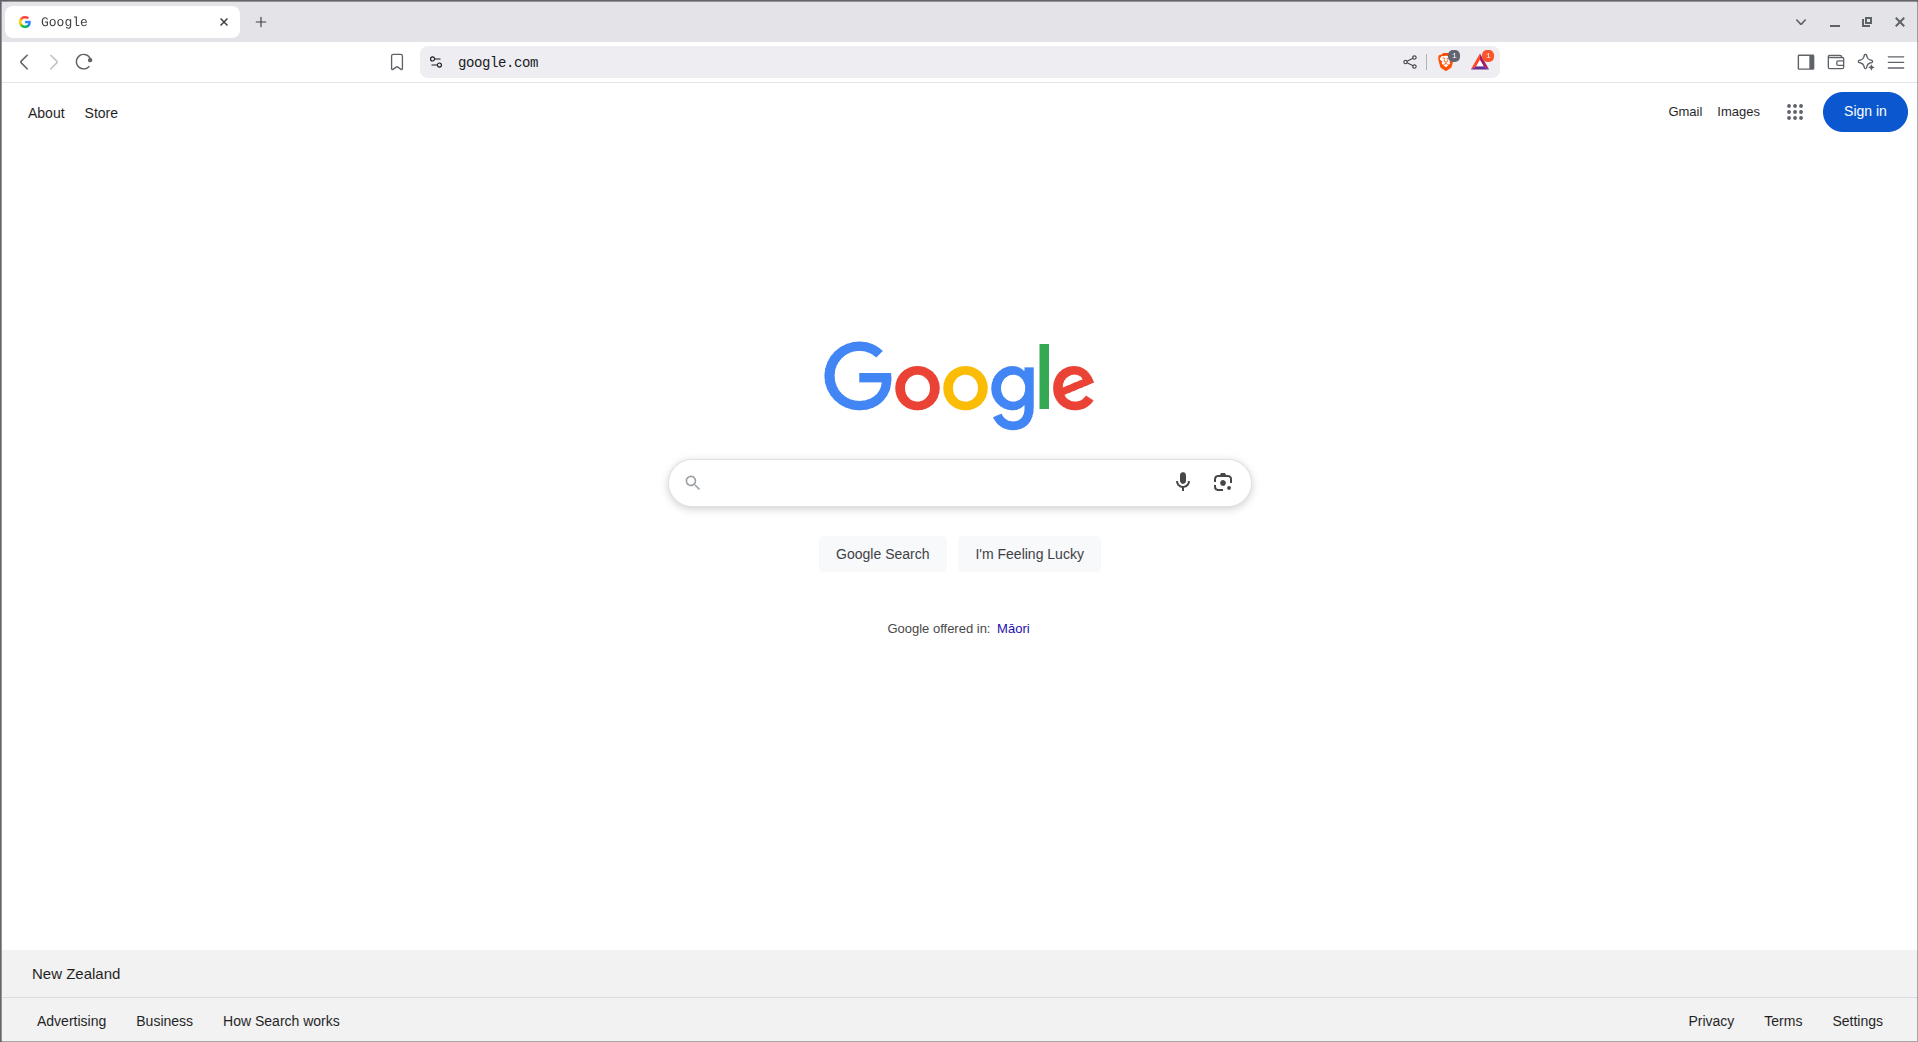
\includegraphics[width=0.8\textwidth]{proto-brave}
    \caption{Brave Browser in Container}
    \label{fig:proto-brave}
\end{figure}

\subsubsection{Prototype 2 (Wine)}
Wine is a state of art application which is developed to run Windows application on Linux kernel with seamless design. In this prototype Winbox (MikorTik Router Management Software) will  run on top of wine.

\begin{lstlisting}[language=Bash]
FROM alpine:latest as downloader
RUN apk add curl
RUN curl -JL https://download.mikrotik.com/routeros/winbox/3.41/winbox64.exe -o winbox.exe

FROM fedora:latest

RUN yum install wine -y --setopt=install_weak_deps=False \
    && yum clean all \
    && rm -rf /var/cache/yum \
    && find / -xdev -type f -perm /u+s -exec chmod -c u-s {} \; \
    && find / -xdev -type f -perm /g+s -exec chmod -c g-s {} \;

COPY --from=downloader --chown=user:user /winbox.exe /

WORKDIR /home/ubuntu

ENTRYPOINT [ "/usr/bin/wine","/winbox.exe" ]
\end{lstlisting}

And it can be built and run with 
\begin{lstlisting}[language=Bash]
podman build -t winbox -f Containerfile .
podman run \
    --rm \
    --userns=keep-id \
    --group-add=video \
    --device=/dev/kfd \
    --device=/dev/dri \ 
    -e XDG_CURRENT_DESKTOP \
    -e DISPLAY \
    -v /tmp/.X11-unix:/tmp/.X11-unix
    --transient-store \
    winbox
\end{lstlisting}

\begin{figure}[ht]
    \centering
    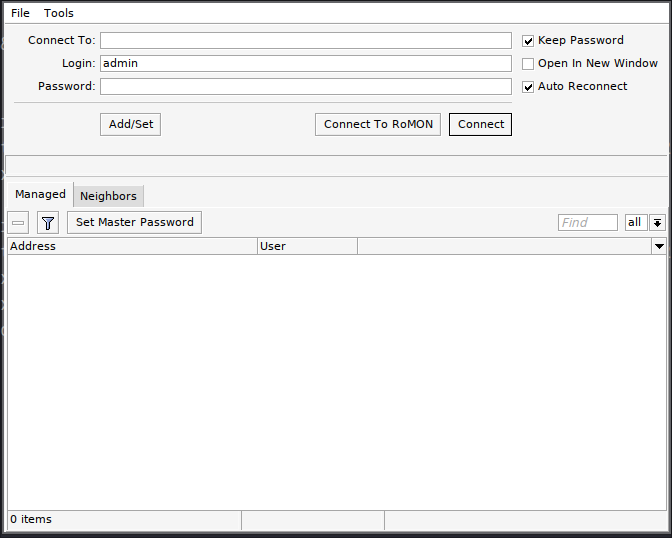
\includegraphics[width=0.5\textwidth]{proto-winbox}
    \caption{Winbox on wine in Container}
    \label{fig:proto-winbox}
\end{figure}

Unlike the first prototype the Winbox in wine is running with X11 display server and the container base is Fedora.

\newpage
\subsubsection{Prototype 3 (Obsidian)}
Obsidian is note taking app based on electron. This is a sample prototype for all electron based applications.

\begin{lstlisting}[language=Bash]
FROM alpine:latest as downloader
RUN apk add curl
RUN curl -JLO $(curl -s https://api.github.com/repos/obsidianmd/obsidian-releases/releases | grep -E ".*url.*amd64.deb" | cut -d '"' -f4 | head -1)

FROM ubuntu:latest

COPY --from=downloader --chown=ubuntu:ubuntu /obsidian* /obsidian.deb

RUN apt update && apt install -yq --no-install-recommends\
        libdrm2 \
        libgbm1 \
        libasound2t64 \
        libgtk-3-0 \
        libnotify4 \
        libnss3 \
        libxss1 \
        libxtst6 \
        xdg-utils \
        libatspi2.0-0 \
        libsecret-1-0 \
        ffmpeg \
        /obsidian.deb \
    && fc-cache -fv \
    && rm -rf /var/lib/apt/lists/* \
    && apt autoclean && apt autoremove --purge && apt clean \
    && find / -xdev -type f -perm /u+s -exec chmod -c u-s {} \; \
    && find / -xdev -type f -perm /g+s -exec chmod -c g-s {} \; \
    && rm -rf /obsidian.deb

ENTRYPOINT [ "obsidian" ]
\end{lstlisting}
\newpage
And the command to build and run is
\begin{lstlisting}[language=Bash]
podman build -t obsidian -f Containerfile .
podman run
    --rm \
    --userns=keep-id \
    --group-add=video \
    --device=/dev/kfd \
    --device=/dev/dri \ 
    -e XDG_CURRENT_DESKTOP \
    -e DISPLAY \
    -v /tmp/.X11-unix:/tmp/.X11-unix
    obsidian 
\end{lstlisting}

\begin{figure}[ht]
    \centering
    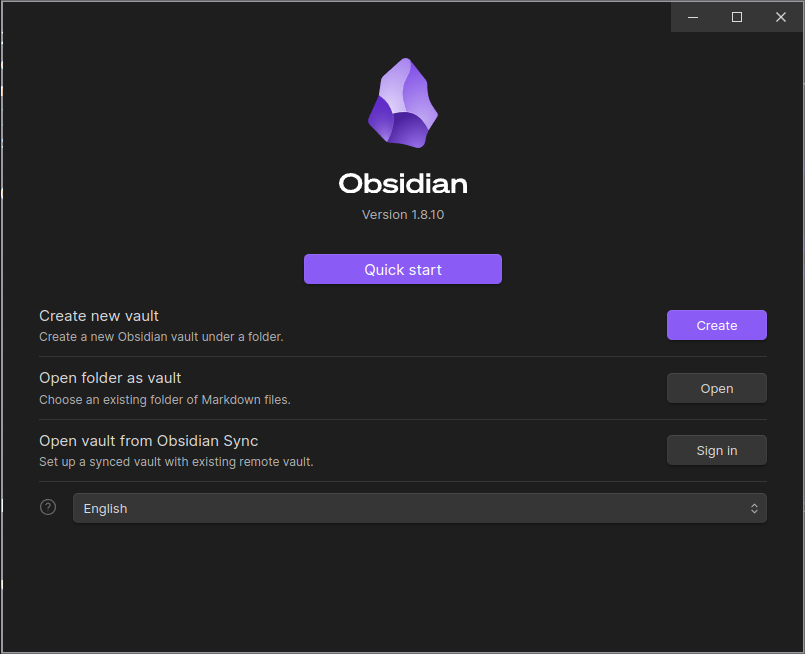
\includegraphics[width=0.5\textwidth]{proto-obsidian}
    \caption{Obsidian in Container}
    \label{fig:proto-obsidian}
\end{figure}

\subsubsection{Prototype 4 (Zoom)}
Zoom is a popular meeting software and it is based on QT library for graphic.

\begin{lstlisting}[language=Bash]
FROM alpine:latest as downloader
RUN apk add curl
RUN curl -J -L -O https://zoom.us/client/latest/zoom_amd64.deb

FROM ubuntu:latest

COPY --from=downloader --chown=1000:1000 /zoom_amd64.deb /zoom_amd64.deb

RUN apt update && apt install -yq --no-install-recommends \
        libnss3 \
        libasound2t64 \
        libpulse0 \
        qt5dxcb-plugin \
        /zoom_amd64.deb \
    && fc-cache -fv \
    && rm -rf /var/lib/apt/lists/* \
    && apt autoclean && apt autoremove --purge && apt clean \
    && find / -xdev -type f -perm /u+s -exec chmod -c u-s {} \; \
    && find / -xdev -type f -perm /g+s -exec chmod -c g-s {} \; \
    && echo "default-server = unix:/run/user/1000/pulse/native\nautospawn = no\ndaemon-binary = /bin/true\nenable-shm = false" > /etc/pulse/client.conf

ENTRYPOINT [ "zoom" ]
\end{lstlisting}
\newpage
And the command to build and run is
\begin{lstlisting}[language=Bash]
podman build -t zoom -f Containerfile .
podman run
    --rm \
    --userns=keep-id \
    --group-add=video \
    --device=/dev/kfd \
    --device=/dev/dri \ 
    -e XDG_CURRENT_DESKTOP \
    -e XDG_RUNTIME_DIR \
    -e WAYLAND_DISPLAY \
    -v ${XDG_RUNTIME_DIR}/${WAYLAND_DISPLAY}:${XDG_RUNTIME_DIR}/${WAYLAND_DISPLAY} \
    -v ${XDG_RUNTIME_DIR}/pulse:${XDG_RUNTIME_DIR}/pulse \
    --transient-store \
    zoom
\end{lstlisting}

Zoom application is specifically chose for prototype to demonstrate other peripheral functions such as camera and microphone.

\begin{figure}[ht]
    \centering
    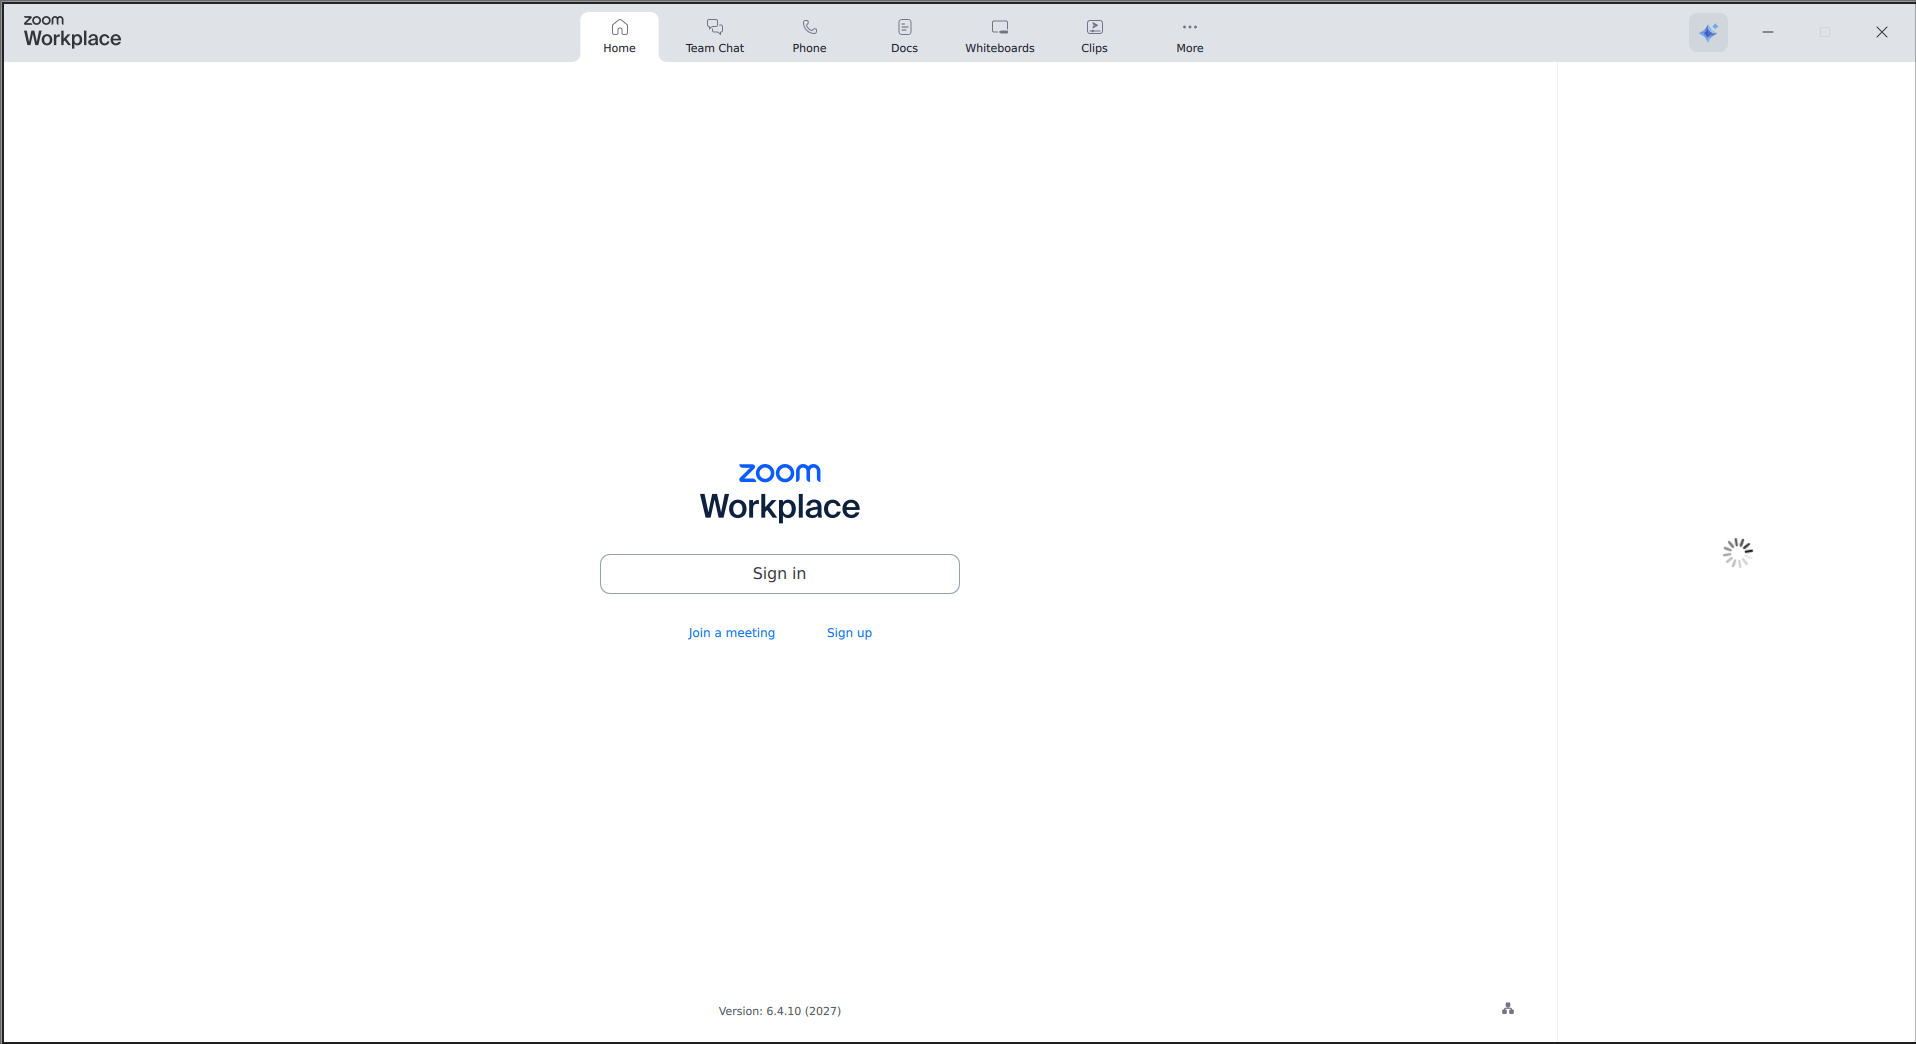
\includegraphics[width=0.8\textwidth]{proto-zoom}
    \caption{Zoom in Container}
    \label{fig:proto-zoom}
\end{figure}

\subsubsection{Prototype 5 (Tor Browser)}
For the last prototype, we will demonstrate with Tor Browser, a privacy oriented Firefox based browser which is based on GTK library for graphic.

\begin{lstlisting}[language=Bash]
FROM alpine:latest as downloader
RUN apk add curl jq
RUN curl -fssLO $(curl https://aus1.torproject.org/torbrowser/update_3/release/downloads.json | jq -r '.downloads."linux-x86_64".ALL.binary') \
    && tar xvf tor-browser-*

FROM ubuntu:latest
RUN apt update && apt install -yq --no-install-recommends \
        keyboard-configuration \
        libx11-xcb1 \
        libxt6 \
        libgtk-3-0 \
        libdbus-glib-1-2 \
        file \
        libpulse0 \
        libasound2t64 \
    && fc-cache -fv \
    && rm -rf /var/lib/apt/lists/* \
    && apt autoclean && apt autoremove --purge && apt clean \
    && find / -xdev -type f -perm /u+s -exec chmod -c u-s {} \; \
    && find / -xdev -type f -perm /g+s -exec chmod -c g-s {} \; \
    && echo "default-server = unix:/run/user/1000/pulse/native\nautospawn = no\ndaemon-binary = /bin/true\nenable-shm = false" > /etc/pulse/client.conf

COPY --from=downloader --chown=1000:1000 /tor-browser/ /tor

ENTRYPOINT [ "/tor/Browser/start-tor-browser" ]
\end{lstlisting}

And the command to build and run is
\begin{lstlisting}[language=Bash]
podman build -t tor-browser -f Containerfile .
podman run
    --rm \
    --userns=keep-id \
    --group-add=video \
    --device=/dev/kfd \
    --device=/dev/dri \ 
    -e XDG_CURRENT_DESKTOP \
    -e XDG_RUNTIME_DIR \
    -e WAYLAND_DISPLAY \
    -e MOZ_ENABLE_WAYLAND=1 \
    -v ${XDG_RUNTIME_DIR}/${WAYLAND_DISPLAY}:${XDG_RUNTIME_DIR}/${WAYLAND_DISPLAY} \
    -v ${XDG_RUNTIME_DIR}/pulse:${XDG_RUNTIME_DIR}/pulse \
    --transient-store \
    tor-browser
\end{lstlisting}

The flag \code{-e MOZ\_ENABLE\_WAYLAND=1} is specifically added to force the browser to run on Wayland mode.

\begin{figure}[ht]
    \centering
    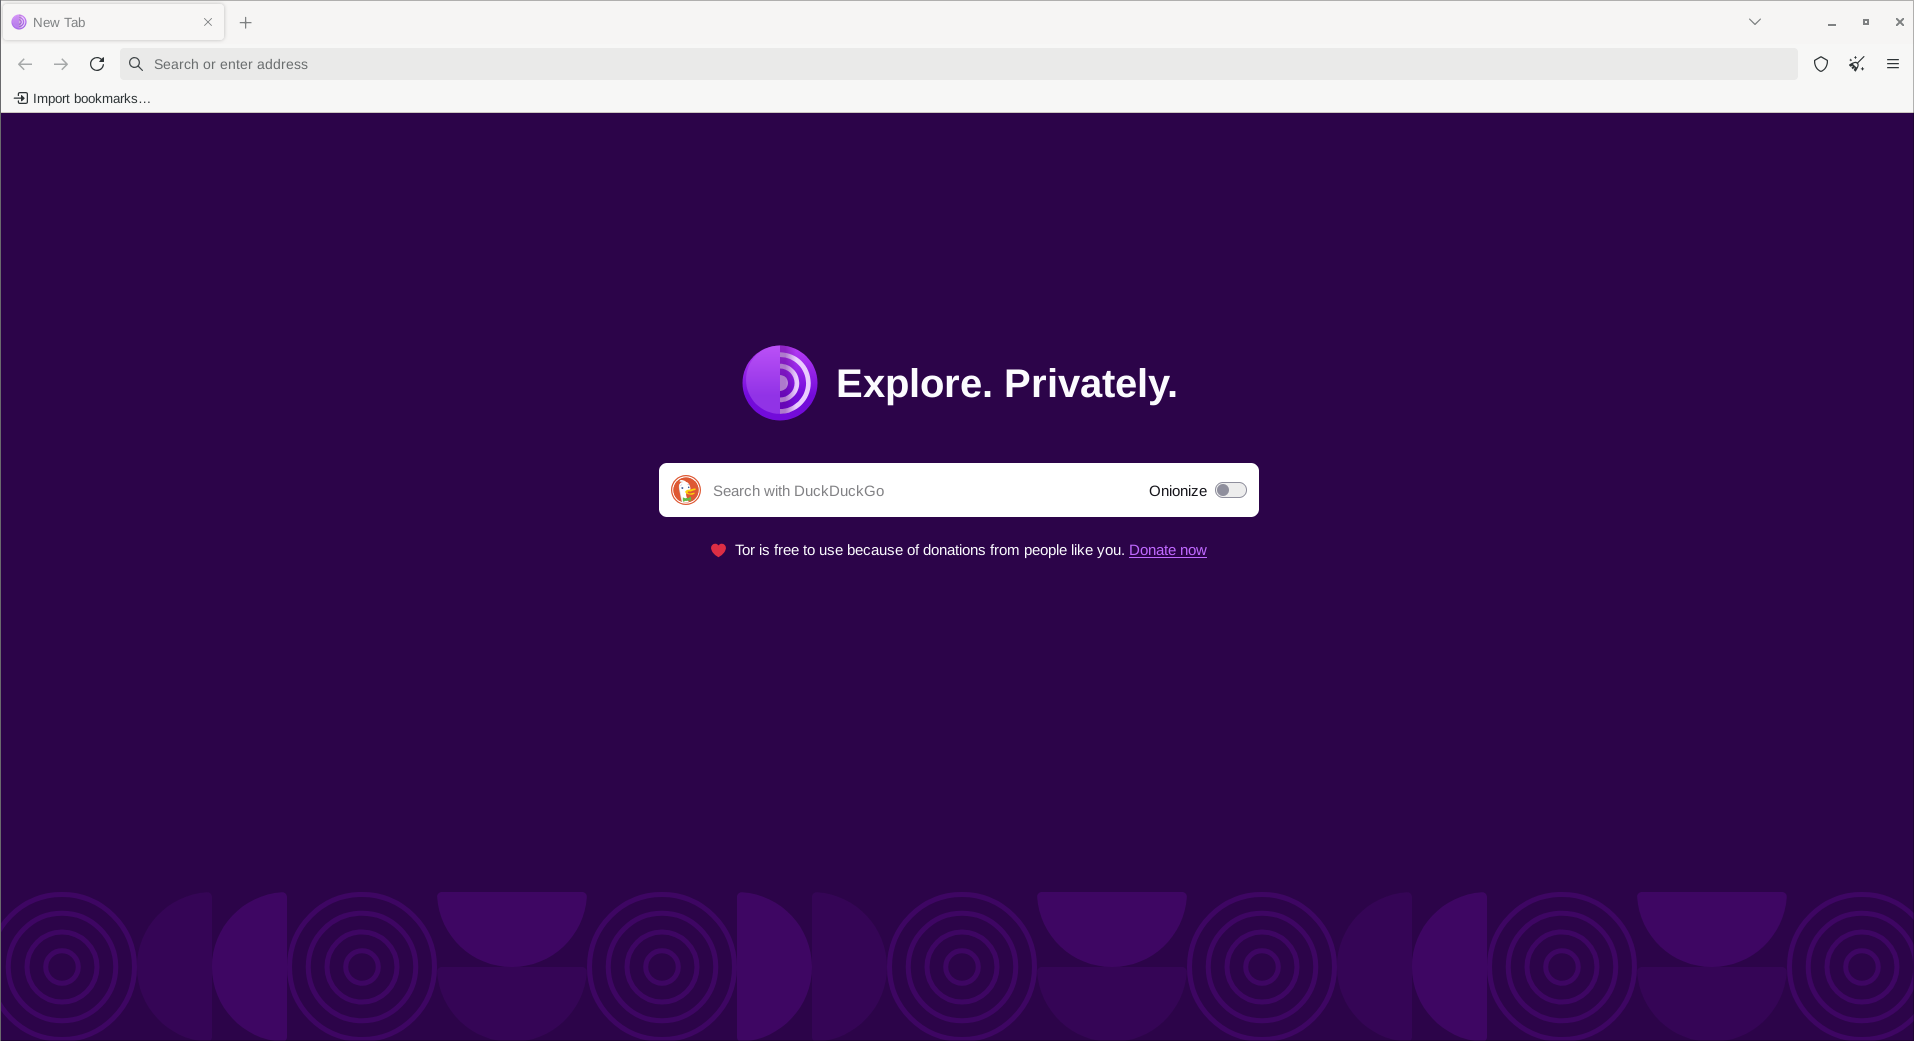
\includegraphics[width=0.8\textwidth]{proto-tor}
    \caption{Tor Browser in Container}
    \label{fig:proto-tor}
\end{figure}
The above prototypes are samples demonstrations using Podman container to run various applications with different configurations and environments.

\newpage
\section{Findings, Analysis and Evaluation}
The results of the study are directly linked to the research problems which are mentioned in the introduction and research questions.

\subsection{Findings}
\subsubsection{Mitigation of Host-Level Dependency Issues (Addressing RQ1)}
The development and successful execution of diverse GUI applications within containers demonstrated a significant mitigation of the "dependency hell" problem at the host operating system level. By encapsulating applications and their specific library dependencies within the container image (Containerfiles explicitly listed required libraries like libgl1, libpulse0, libegl1-mesa, libnss3, libasound2t64, libgtk-3-0, etc.), the research confirmed that applications could run independently of the host distribution's installed library versions or packaging system. This approach effectively decouples the application from the host environment's dependency chain, allowing the same container image to theoretically run on any Linux distribution capable of running the container runtime (Podman), provided the necessary host-level integration points (display server, audio, devices) are accessible.

However, dependency management is not eliminated but rather shifted to the container image build process which means the dependency management is shifted to developer. Developers must now define and manage dependencies within the Containerfile. This solution is logical since the developer has the exact knowledge of which packages are required for the application developed.

\subsubsection{Security Implications and Integration Challenges (Addressing RQ2)}

Containerisation inherently provides a layer of isolation using Linux kernel features like namespaces and cgroups. This isolates the application's file-system, processes, and network from the host system to a significant degree, improving security compared to natively installing potentially untrusted software directly onto the host. The use of user namespaces (--userns=keep-id) in the prototypes further enhanced security by preventing the container process from running as root on the host. Normalising file permissions within the container image also contributed to a more secure default posture.

However, integrating GUI applications necessitates granting the container access to host resources such as the display server (X11 or Wayland sockets), audio system (PulseAudio socket), and graphics hardware (/dev/dri, /dev/kfd, --group-add=video). These access points represent potential vectors for security vulnerabilities if the containerised application is compromised. But in this hypothetical scenario, if the bad actors can successfully infiltrate the application inside the container, they definitely can penetrate the application inside the host layer. Comparing to the native layer, the container gives extra layer to halt the attack. 

To partially mitigate the potential security vulnerability, the container support more more granular security policies (e.g., Seccomp profiles, AppArmor/SELinux policies specific to containerised GUI apps) to the risks introduced in the container's isolation.

\subsubsection{Design Considerations and End-User Experience Impact (Addressing RQ3)}

The prototype development process shows several key design considerations for a container-based application packaging system:

Image Structure: Images need to include the application binary and all its runtime dependencies not provided by a minimal base image. Multi-stage builds (used in Prototypes 2, 3, 4, 5) are effective for separating build dependencies from runtime dependencies and minimising final image size.
Dependency Management: Shifting dependency management to the Containerfile requires a clear definition of required libraries for each application. Using a robust base image (like Ubuntu in most prototypes) simplifies this by providing common libraries, but increases image size.
Host Integration: Robust mechanisms are required to handle the variability of host display servers (X11 vs. Wayland), audio systems, and hardware access. The prototype Podman run commands demonstrate the complexity involved, requiring specific volume mounts, environment variables, and device/group access flags. A user-friendly system would need to abstract this complexity.
Persistence: While --transient-store was used for quick testing, a real system requires a strategy for persistent user data and configuration (e.g., using named volumes).

At the current stage,  applications are portable across different Linux distributions without host dependency conflicts. Installation conceptually becomes pulling/building a single image. But there are some underdeveloped parts such as the command (Podman run with numerous flags for display, audio, devices, user namespaces, etc.) is significantly more complex than simply typing an application name or clicking an icon. Integration with the host desktop environment (e.g., file pickers, system notifications, theme consistency) was not fully seamless within the scope of the prototypes and represents a major usability challenge for a general-purpose desktop application delivery system.

\subsection{Analysis}
This section provides a detailed analysis and interpretation of the findings.

\subsubsection{Analysis of Dependency Mitigation}
The findings shows that containerisation offers a robust solution to the "dependency hell" problem at the host operating system level. By bundling the application and dependencies within the container image, the approach decouples the application's runtime environment from the host distribution's library (e.g., APT, YUM/DNF). This was demonstrated by the ability of the same container images (e.g., the Brave Browser container based on Ubuntu) to run on different host distributions without encountering library conflicts or requiring specific host package installations beyond the container runtime itself.

\subsubsection{Analysis of Superiority}
Compared to traditional methods, this approach eliminates the need for complex dependency algorithms on the host (as discussed in relation to OPIUM\cite{10.1109/ICSE.2007.59}) and avoids the potential for system-wide library version clashes. Unlike universal package formats like Flatpak or Snap, which also provide isolation, the container approach leverages standard container runtime and image formats (OCI-compliant), potentially offering broader compatibility with existing container infrastructure and workflows

\subsubsection{Analysis of Security}
The container isolation utilise Linux kernel features like namespaces and cgroups, offers a significant security advantage compared to installing potentially untrusted applications directly onto the host system. The prototypes demonstrated effective isolation of the application's filesystem and processes. The findings point out that if an attacker can compromise the application inside the container, they might also be able to compromise it if installed natively. The container's isolation aims to confine the damage, preventing easy lateral movement or access to the entire host system, unlike a native application with full user privileges.

\subsubsection{Analysis of Design and End-User Experience}
The prototype development process demonstrate design considerations for building a container-based packaging system for a comprehensive Linux environment. One of the main improvement is the image structure, where multi-stage builds minimise final image size by separating build dependencies from runtime requirements. Managing application dependencies shifts entirely to the Containerfile, requiring developers to accurately define and maintain the required libraries.

Figure 6 shows some user from different backgrounds giving feedback from using the containerised applications of noticible difference in startup time.
\begin{figure}[ht]
    \centering
    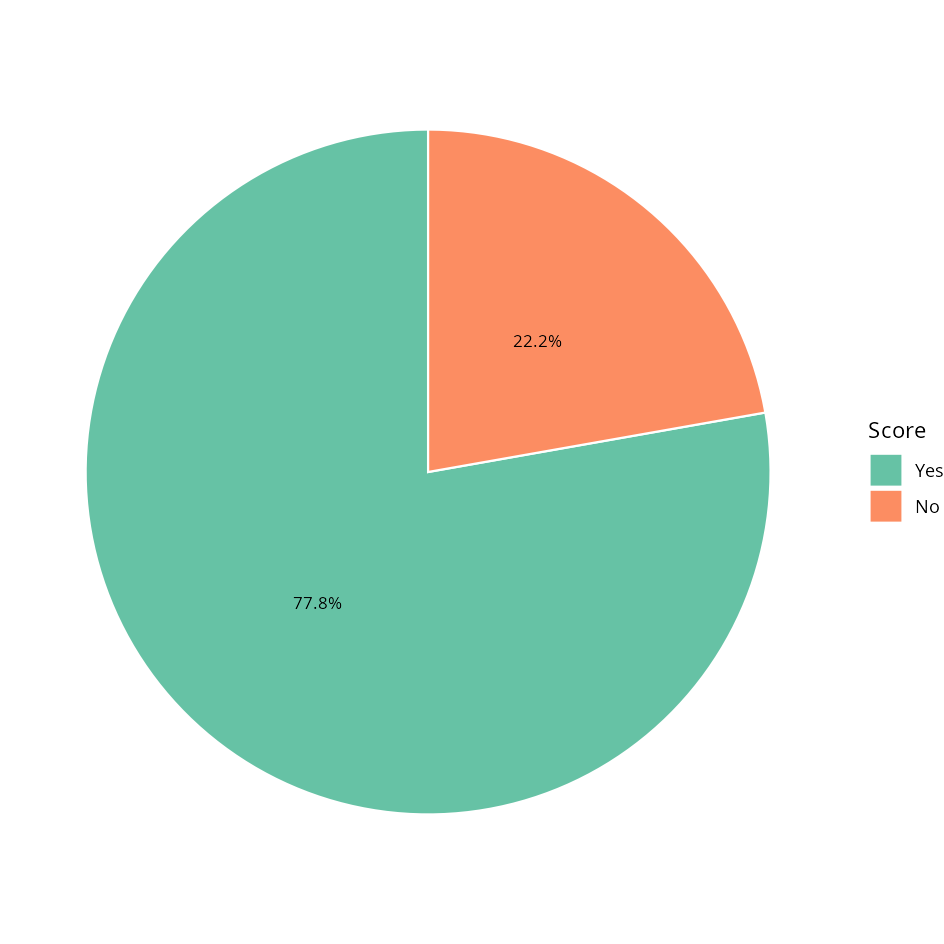
\includegraphics[width=0.4\textwidth]{pie_ui2}
    \caption{Performance Difference Survey}
    \label{fig:pi_ui2}
\end{figure}

\newpage
\subsubsection{Analysis of Performance Metrics}
Startup Time: Figure 7 illustrates the startup time comparison between native installations and containerised executions for the selected applications (Brave Browser, Zoom, Winbox/Wine).
\begin{figure}[ht!]
    \centering
    \subfloat[Brave Browser\label{1a}]{%
    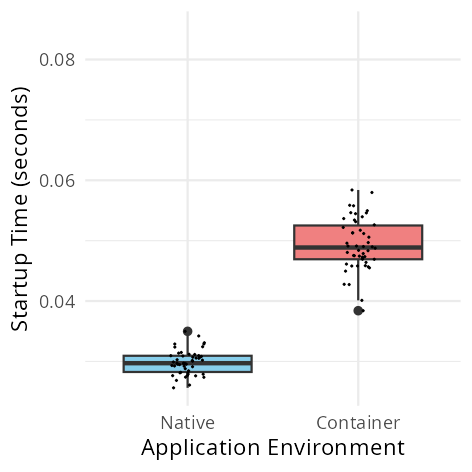
\includegraphics[width=0.3\linewidth]{startup_brave}}
    \hfill
    \subfloat[Zoom\label{1b}]{%
    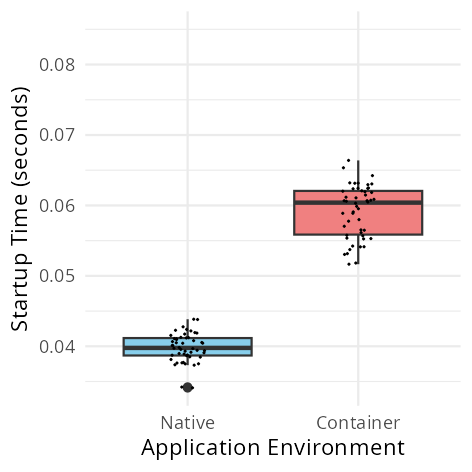
\includegraphics[width=0.3\linewidth]{startup_zoom}}
    \hfill
    \subfloat[Winbox(Wine)\label{1c}]{%
    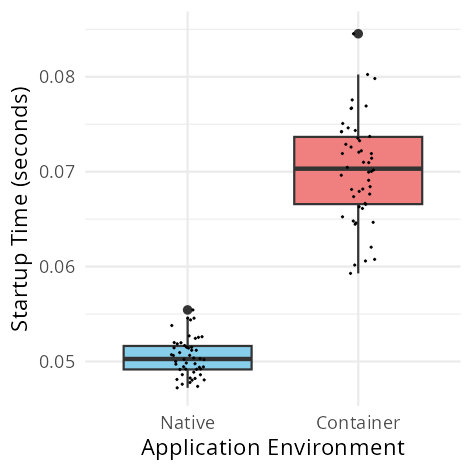
\includegraphics[width=0.3\linewidth]{startup_winbox}}
    \caption{Startup Time Comparison}
\end{figure}

The Figure 7 indicate there are some container overhead delay for each applications. But the difference is only in the sub mill-second region which is not noticeable by end user. During the demonstration, the \code{--transient-store} flag is used to lessen the page storage size which might have some effect on the startup time.

As shown in Figure 8, the survey results indicate whether different users notice the difference between native and containerised application.

\begin{figure}[ht]
    \centering
    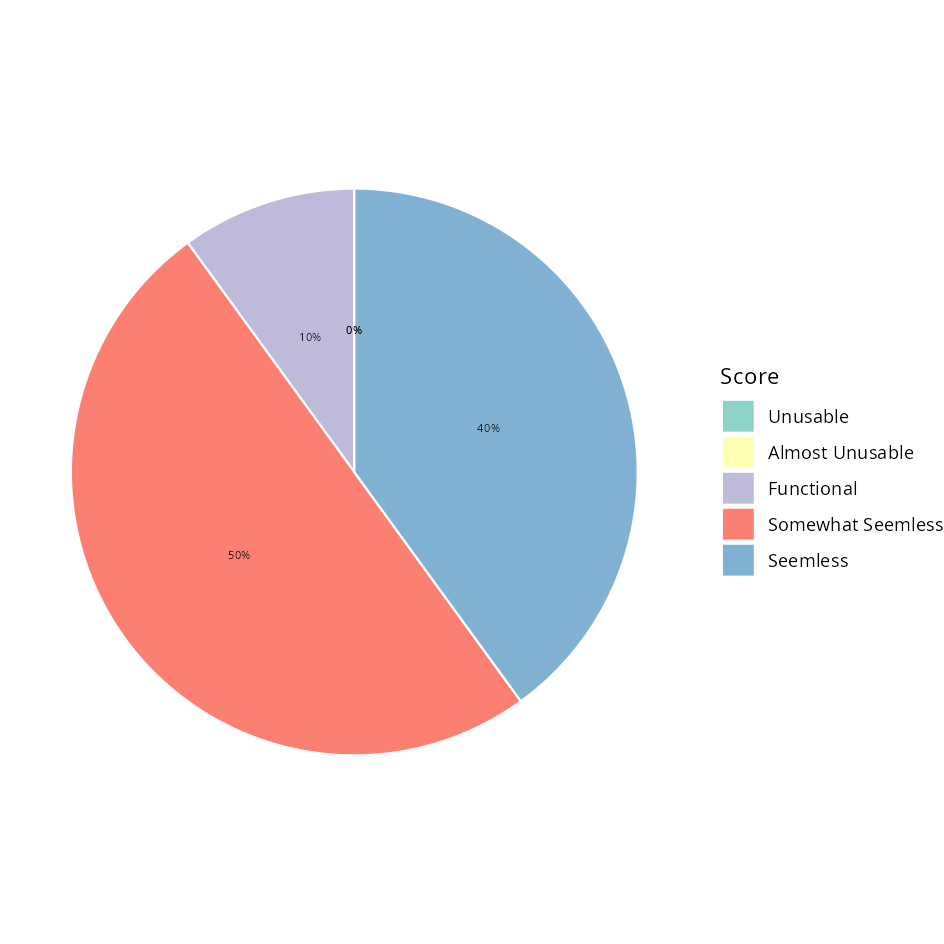
\includegraphics[width=0.4\textwidth]{pie_ui}
    \caption{Startup Time Difference Survey}
    \label{fig:pi_ui}
\end{figure}
\newpage
RAM Usage: Figure 8 presents the RAM usage comparison between native and containerised applications (Brave Browser, Zoom, Winbox/Wine).

\begin{figure}[ht!]
    \centering
    \subfloat[Brave Browser\label{2a}]{%
    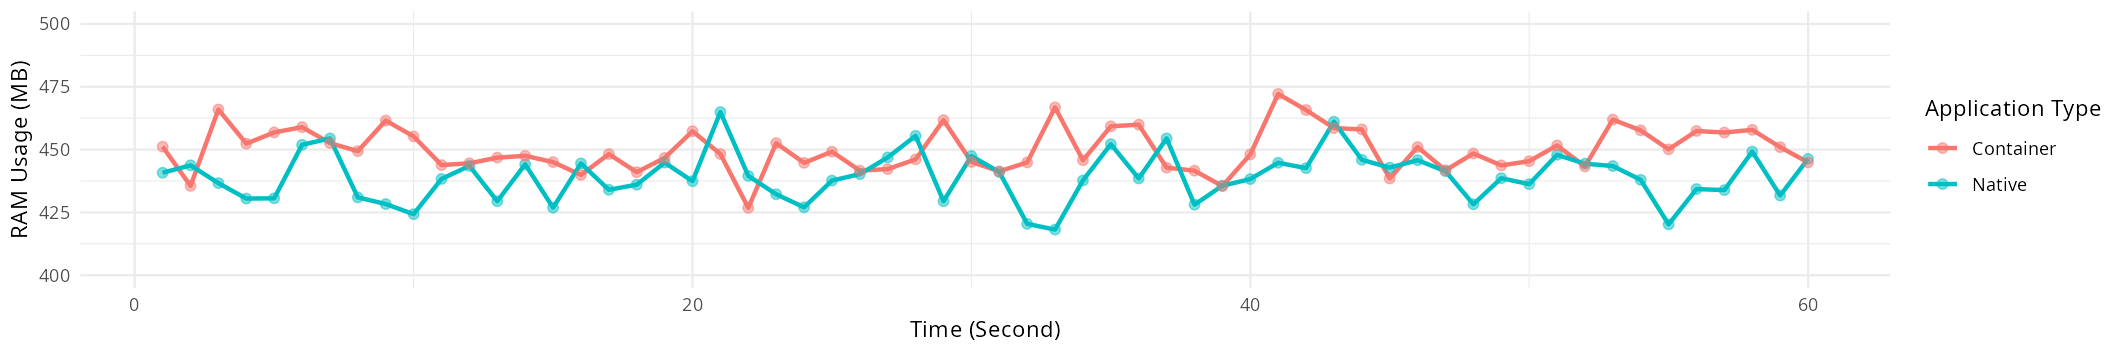
\includegraphics[width=1\linewidth]{ram_brave}}
    \hfill
    \\
    \subfloat[Zoom\label{2b}]{%
    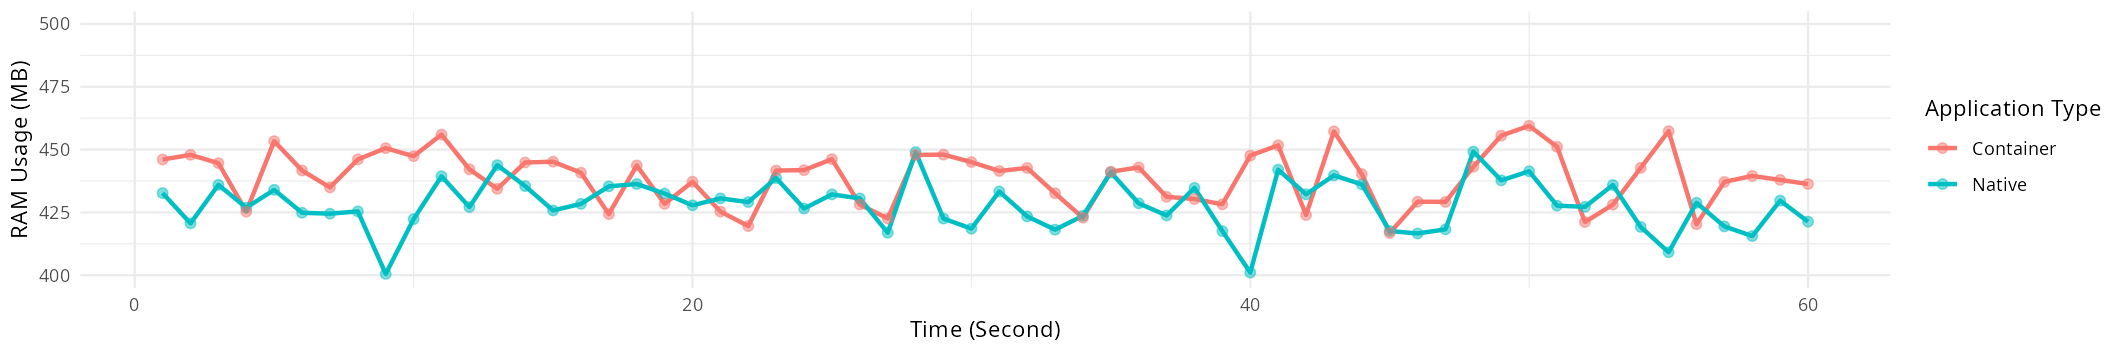
\includegraphics[width=1\linewidth]{ram_zoom}}
    \hfill
    \\
    \subfloat[Winbox(Wine)\label{2c}]{%
    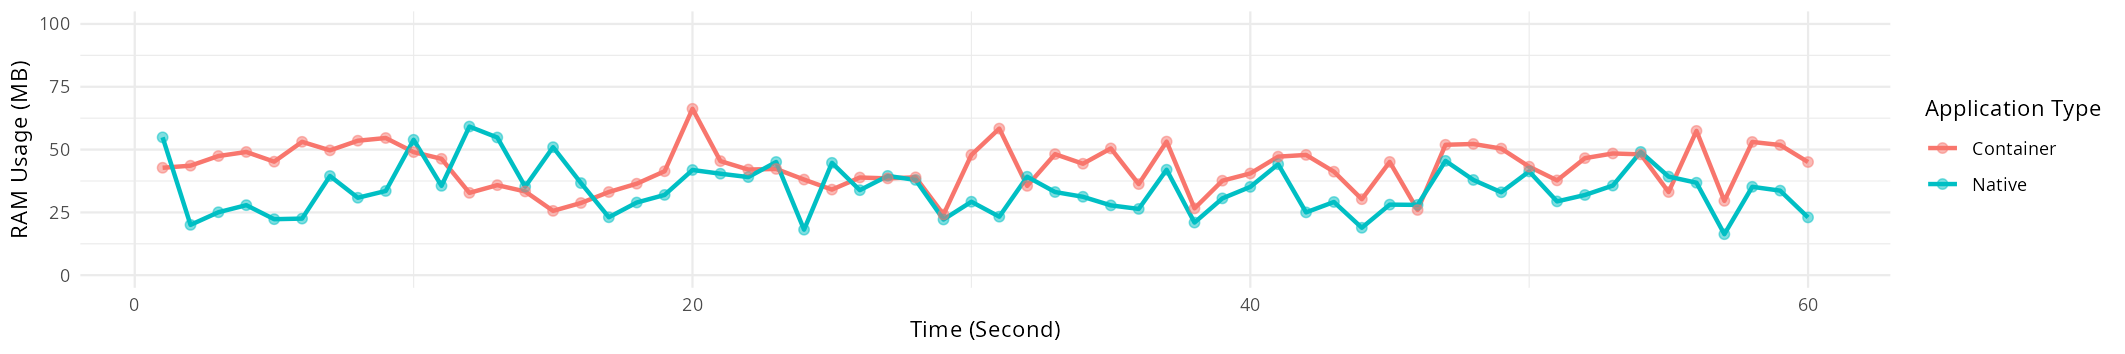
\includegraphics[width=1\linewidth]{ram_winbox}}
    \caption{RAM Usage Comparison}
\end{figure}

Regarding RAM usage, no significant difference was found between the native and container versions of the applications. Sudden dips were observed in the native version but not in the container version, suggesting that the container environment regulates RAM usage to maintain a consistent level.

Overall, the performance analysis suggests that while containerisation offers significant benefits in dependency management and isolation, it may introduce some overhead in startup time and RAM usage compared to highly optimised native installations. These trade-offs must be considered when evaluating the feasibility of a universal container-based system, particularly for performance-sensitive applications or resource-limited environments. The findings align somewhat with the performance trade-offs observed in the Jails vs. Docker study \cite{Ryding_Johansson_2020}, where different container technologies showed strengths in different performance areas.

\newpage
\section{Conclusion}
The challenge of Linux "dependency hell" rooting form the fragmentation of packaging systems and distribution-specific libraries, significantly hinder application portability and encountering a huge learning curve for new users. This research embarked on the potential of containerisation technology as a unifying system to resolve these issues across every spectrum of Linux branches, mainly complex graphical user interface (GUI) software. Our primary aim was to evaluate the effectiveness of decoupling applications form the host environment using container technology like Podman where offering a consistent and isolated environment.

Our findings validate the effectiveness of encapsulating applications and their required library within a single image. We demonstrated successful running of diverse GUI application across different host environments. For security, we explained the containers inherently offer a layer of isolation compared to native installation using through kernel features. We managed to shared the host resources such as display server, audio and devices where the container isolation layer still provides a border for outer attacks by utilising granular security policies.

From a design perspective, we constructed efficient images, leveraging multi-stage builds to minimise size, and developing robust, abstracted mechanisms for host resource integration. Performance analysis indicated that while containerisation introduces some minimal overhead in application startup time and potentially affects RAM usage consistency compared to highly optimised native installations, these differences were largely imperceptible to users which is suggesting that the performance cost is an acceptable trade-off for the benefits gained in dependency management and isolation.

The implications of these findings are significant for the future of Linux application distribution which can enable developers to target a single, containerised format that runs consistently across virtually any Linux distribution. This could accelerate software availability, simplify maintenance, and provide a more stable user experience by eliminating dependency conflicts.

Future research should focus on developing a user-friendly script or daemon that reduce complexities of container execution and host resource sharing which enable seamless application launching and deeper desktop integration. Further work is also needed to define standard security policies and best practices specifically tailored for containerised GUI applications to maximise isolation while maintaining necessary functionality. More extensive performance benchmarking across a wider range of hardware and application types would provide a deeper understanding of the performance trade-offs. Finally, exploring mechanisms for updates and distribution of containerised applications, using existing container registries, will be important for building a practical and scalable ecosystem. This study provides a strong foundation for exploring containerisation as a fundamental shift in Linux application delivery.

\newpage
% needed in second column of first page if using \IEEEpubid
%\IEEEpubidadjcol

% \subsubsection{Subsubsection Heading Here}
% Subsubsection text here.


% An example of a floating figure using the graphicx package.
% Note that \label must occur AFTER (or within) \caption.
% For figures, \caption should occur after the \includegraphics.
% Note that IEEEtran v1.7 and later has special internal code that
% is designed to preserve the operation of \label within \caption
% even when the captionsoff option is in effect. However, because
% of issues like this, it may be the safest practice to put all your
% \label just after \caption rather than within \caption{}.
%
% Reminder: the "draftcls" or "draftclsnofoot", not "draft", class
% option should be used if it is desired that the figures are to be
% displayed while in draft mode.
%
%\begin{figure}[!t]
%\centering
%\includegraphics[width=2.5in]{myfigure}
% where an .eps filename suffix will be assumed under latex, 
% and a .pdf suffix will be assumed for pdflatex; or what has been declared
% via \DeclareGraphicsExtensions.
%\caption{Simulation results for the network.}
%\label{fig_sim}
%\end{figure}

% Note that the IEEE typically puts floats only at the top, even when this
% results in a large percentage of a column being occupied by floats.


% An example of a double column floating figure using two subfigures.
% (The subfig.sty package must be loaded for this to work.)
% The subfigure \label commands are set within each subfloat command,
% and the \label for the overall figure must come after \caption.
% \hfil is used as a separator to get equal spacing.
% Watch out that the combined width of all the subfigures on a 
% line do not exceed the text width or a line break will occur.
%
%\begin{figure*}[!t]
%\centering
%\subfloat[Case I]{\includegraphics[width=2.5in]{box}%
%\label{fig_first_case}}
%\hfil
%\subfloat[Case II]{\includegraphics[width=2.5in]{box}%
%\label{fig_second_case}}
%\caption{Simulation results for the network.}
%\label{fig_sim}
%\end{figure*}
%
% Note that often IEEE papers with subfigures do not employ subfigure
% captions (using the optional argument to \subfloat[]), but instead will
% reference/describe all of them (a), (b), etc., within the main caption.
% Be aware that for subfig.sty to generate the (a), (b), etc., subfigure
% labels, the optional argument to \subfloat must be present. If a
% subcaption is not desired, just leave its contents blank,
% e.g., \subfloat[].


% An example of a floating table. Note that, for IEEE style tables, the
% \caption command should come BEFORE the table and, given that table
% captions serve much like titles, are usually capitalized except for words
% such as a, an, and, as, at, but, by, for, in, nor, of, on, or, the, to
% and up, which are usually not capitalized unless they are the first or
% last word of the caption. Table text will default to \footnotesize as
% the IEEE normally uses this smaller font for tables.
% The \label must come after \caption as always.
%
%\begin{table}[!t]
%% increase table row spacing, adjust to taste
%\renewcommand{\arraystretch}{1.3}
% if using array.sty, it might be a good idea to tweak the value of
% \extrarowheight as needed to properly center the text within the cells
%\caption{An Example of a Table}
%\label{table_example}
%\centering
%% Some packages, such as MDW tools, offer better commands for making tables
%% than the plain LaTeX2e tabular which is used here.
%\begin{tabular}{|c||c|}
%\hline
%One & Two\\
%\hline
%Three & Four\\
%\hline
%\end{tabular}
%\end{table}


% Note that the IEEE does not put floats in the very first column
% - or typically anywhere on the first page for that matter. Also,
% in-text middle ("here") positioning is typically not used, but it
% is allowed and encouraged for Computer Society conferences (but
% not Computer Society journals). Most IEEE journals/conferences use
% top floats exclusively. 
% Note that, LaTeX2e, unlike IEEE journals/conferences, places
% footnotes above bottom floats. This can be corrected via the
% \fnbelowfloat command of the stfloats package.









% if have a single appendix:
%\appendix[Proof of the Zonklar Equations]
% or
%\appendix  % for no appendix heading
% do not use \section anymore after \appendix, only \section*
% is possibly needed

% use appendices with more than one appendix
% then use \section to start each appendix
% you must declare a \section before using any
% \subsection or using \label (\appendices by itself
% starts a section numbered zero.)
%


\appendices
\section{Other Containerfile Prototypes and Execution Commands}
OBS Containerfile

\begin{lstlisting}[language=Bash]
FROM ubuntu:latest

RUN groupadd -g 1000 -r user \
    && useradd -u 1000 -s /bin/bash -r -G audio,video -g 1000 -m user

RUN apt update && apt install -yq --no-install-recommends \
        keyboard-configuration \
        software-properties-common \
        gpg-agent \
        ffmpeg \
        libpulse0 \
    && add-apt-repository -y ppa:obsproject/obs-studio \
    && apt update \
    && apt install -yq --no-install-recommends obs-studio \
    && fc-cache -fv \
    && rm -rf /var/lib/apt/lists/* \
    && apt autoclean && apt autoremove --purge && apt clean \
    && find / -xdev -type f -perm /u+s -exec chmod -c u-s {} \; \
    && find / -xdev -type f -perm /g+s -exec chmod -c g-s {} \; \
    && echo "default-server = unix:/run/user/1000/pulse/native\nautospawn = no\ndaemon-binary = /bin/true\nenable-shm = false" > /etc/pulse/client.conf

USER user

WORKDIR /home/user

ENTRYPOINT [ "obs" ]

\end{lstlisting}

Sample Container Image Builder
\begin{lstlisting}[language=Bash]
#!/bin/bash

BUILDER=podman

x=("brave" "gtkcord4" "libreoffice" "librewolf" "mullvad-browser" "obs" "qbittorrent" "staruml" "telegram" "tor" "ungoogled-chromium" "winbox" "zoom")

if [ "$1" = "selected" ] ; then
    for f in ${x[@]} ; do
        echo "=-------------------------------------->"
        echo "|"
        echo "|-----> Building $f"
        echo "|"
        echo "=-------------------------------------->"
        ${BUILDER} build -t peterzam/box-$f --no-cache -f https://codeberg.org/peterzam/box/raw/branch/main/$f/Containerfile .
    done
else
    ${BUILDER} build -t peterzam/box-$1 -f ./$1/Containerfile .
fi
\end{lstlisting}

Sample Runner

\begin{lstlisting}[language=Bash]
#!/bin/bash

if [ $# -le 1 ] || [ ${1:0:1} != '-' ]
then
    echo -e "Specify Display type"
    echo -e "Usage: \n-x (use X11 display) \n-w (use Wayland display)" >&2
    exit 1
fi


### Runner ###
runner='podman'

### Box ###
box=$2

### BOX PATH ###
BOXPATH='
/home/p/custom/box-mounts'


### name ###
NAME='
--name='${box}'-box-'${RANDOM}

### Remove ###
RM='
--rm'

### User ###
USERNS='
--userns=keep-id:gid=1000
--group-add=video' ## for gpu access

### Display ###
DISPLAY_X='
--device=/dev/kfd
--device=/dev/dri
-e DISPLAY
-v /tmp/.X11-unix:/tmp/.X11-unix'

DISPLAY_WAYLAND='
--device=/dev/kfd
--device=/dev/dri
-e XDG_CURRENT_DESKTOP
-e XDG_RUNTIME_DIR
-e WAYLAND_DISPLAY
-v '${XDG_RUNTIME_DIR}'/'${WAYLAND_DISPLAY}':'${XDG_RUNTIME_DIR}'/'${WAYLAND_DISPLAY}

### Audio ###
AUDIO_PULSE='
-v '${XDG_RUNTIME_DIR}'/pulse:'${XDG_RUNTIME_DIR}'/pulse'

### Font ###
FONT='
-v /usr/share/fonts:/usr/share/fonts:ro'

### CHROOT ###
CHROOT='
--cap-add sys_chroot'

### SHM ###
SHM='
--shm-size=2g'

### USB/Serial ###
USB='
-v /dev:/dev --device-cgroup-rule="c 188:* rmw" --device-cgroup-rule="c 81:* rmw"'

### Camera ### #video[int] for other cams
CAMERA='
--device /dev/video0'

### SHARED PATH ###
SHARED='
-v '${BOXPATH}'/shared/'${box}':/home/user/Shared'

###  Transient Storage ###
TRANSIENT='
--transient-store'

### No Network ###
NONET='
--network=none'

### QT WAYLAND###
QT_WAYLAND='
-e QT_QPA_PLATFORM=wayland'

### Mozilla WAYLAND###
MOZILLA_WAYLAND='
-e MOZ_ENABLE_WAYLAND=1'

### Chromium WAYLAND###
CHROMIUM_WAYLAND='
--enable-features=UseOzonePlatform --ozone-platform=wayland'


DEFAULT_DISPLAY=${DISPLAY_WAYLAND}


while getopts 'xwh:' OPTION; do
  case "$OPTION" in
    x)
        DEFAULT_DISPLAY=${DISPLAY_X}
        CHROMIUM_WAYLAND=""
        MOZILLA_WAYLAND=""
        QT_WAYLAND=""
        ;;
    w)
        ;;
    *)
        echo -e "Usage: \n-x (use X11 display) \n-w (use Wayland display)" >&2
        exit 1
        ;;
  esac
done

COMMON="${NAME} ${RM} ${USERNS} ${DEFAULT_DISPLAY} ${SHARED}"

case ${box} in
    brave)
        ${runner} run \
        ${COMMON} ${AUDIO_PULSE} ${TRANSIENT} ${FONT} ${SHM} ${CHROOT} \
        -v ${BOXPATH}/configs/brave:/home/user/.config/BraveSoftware \
        peterzam/box-brave ${CHROMIUM_WAYLAND}
        ;;
    brave-incognito)
        ${runner} run \
        ${COMMON} ${AUDIO_PULSE} ${TRANSIENT} ${SHM} ${CHROOT} \
        peterzam/box-brave ${CHROMIUM_WAYLAND}
        ;;
    gtkcord4)
        ${runner} run \
        ${COMMON} ${FONT} \
        -v ${BOXPATH}/configs/gtkcord4:/home/user/.config/gtkcord4 \
        peterzam/box-gtkcord4
        ;;
    libreoffice)
        ${runner} run \
        ${COMMON} ${AUDIO_PULSE} ${TRANSIENT} ${FONT} \
        peterzam/box-libreoffice
        ;;
    librewolf)
        ${runner} run \
        ${COMMON} ${AUDIO_PULSE} ${TRANSIENT} ${FONT} ${CHROOT} ${MOZILLA_WAYLAND} \
        -v ${BOXPATH}/configs/librewolf:/home/user/.librewolf \
        peterzam/box-librewolf
        ;;
    mullvad-browser)
        ${runner} run \
        ${COMMON} ${AUDIO_PULSE} ${TRANSIENT} ${CHROOT} ${MOZILLA_WAYLAND} \
        peterzam/box-mullvad-browser --verbose # Mullvad Browser run as background process in default
        ;;
    obs)
        ${runner} run \
        ${COMMON} ${AUDIO_PULSE} ${NONET} \
	    -v ${BOXPATH}/configs/obs:/home/user/.config/obs-studio \
        peterzam/box-obs
        ;;
    obsidian)
        ${runner} run -it \
        ${COMMON} ${TRANSIENT} ${NONET} \
	    -v ${BOXPATH}/configs/obsidian:/home/user/.config/obsidian \
        peterzam/box-obsidian
        ;;
    qbittorrent)
        ${runner} run \
        ${COMMON} ${TRANSIENT} ${QT_WAYLAND} \
	    -v ${BOXPATH}/configs/qbittorrent:/home/user/.config/qBittorrent \
        peterzam/box-qbittorrent
        ;;
    staruml)
        ${runner} run \
        ${COMMON} ${FONT} ${SHM} \
        peterzam/box-staruml
        ;;
    telegram)
        ${runner} run \
        ${COMMON} ${AUDIO_PULSE} ${FONT} ${QT_WAYLAND} \
	    -v ${BOXPATH}/configs/telegram:/home/user/.local/share/TelegramDesktop \
        peterzam/box-telegram
        ;;
    tor)
        ${runner} run \
        ${COMMON} ${AUDIO_PULSE} ${TRANSIENT} ${CHROOT} ${MOZILLA_WAYLAND} \
        peterzam/box-tor
        ;;
    ungoogled-chromium)
        ${runner} run \
        ${COMMON} ${AUDIO_PULSE} ${TRANSIENT} ${FONT} ${SHM} ${CHROOT} \
        -v ${BOXPATH}/configs/ungoogled-chromium:/home/user/.config/chromium \
        peterzam/box-ungoogled-chromium ${CHROMIUM_WAYLAND} --disable-top-sites
        ;;
    ungoogled-chromium-incognito)
        ${runner} run \
        ${COMMON} ${AUDIO_PULSE} ${TRANSIENT} ${FONT} ${SHM} ${CHROOT} \
        peterzam/box-ungoogled-chromium ${CHROMIUM_WAYLAND}
        ;;
    winbox)
        ${runner} run \
        ${COMMON} ${TRANSIENT} \
		-v ${BOXPATH}/configs/winbox:/home/user/.wine \
        peterzam/box-winbox
        ;;
    zoom)
        ${runner} run \
        ${COMMON} ${AUDIO_PULSE} ${CHROOT} \
	    -v ${BOXPATH}/configs/zoom/data:/home/user/.zoom \
	    -v ${BOXPATH}/configs/zoom/config:/home/user/.config/ \
        peterzam/box-zoom
        ;;
esac


# Experimental feature - -v ${XDG_RUNTIME_DIR}/pipewire-0:${XDG_RUNTIME_DIR}/pipewire-0 \

\end{lstlisting}

\section{Benchmarking and Survey}
\subsubsection{Benchmarking Methodology Details} 
Exact commands used for measurement (e.g., time -p <command>, htop for peak RAM, specific perf commands).
Used tools : time, htop, perf, grafana, prometheus



\subsection{Podman System Detail}
\begin{lstlisting}[language=Bash]
host:
  arch: amd64
  buildahVersion: 1.40.1
  cgroupControllers:
  - cpu
  - memory
  - pids
  cgroupManager: systemd
  cgroupVersion: v2
  conmon:
    package: conmon-1:2.1.13-1
    path: /usr/bin/conmon
    version: 'conmon version 2.1.13, commit: 82de887596ed8ee6d9b2ee85e4f167f307bb569b'
  cpuUtilization:
    idlePercent: 90.4
    systemPercent: 1.1
    userPercent: 8.5
  cpus: 16
  databaseBackend: sqlite
  distribution:
    distribution: arch
    version: unknown
  eventLogger: journald
  freeLocks: 2047
  hostname: arch
  idMappings:
    gidmap:
    - container_id: 0
      host_id: 1000
      size: 1
    - container_id: 1
      host_id: 100000
      size: 65536
    uidmap:
    - container_id: 0
      host_id: 1000
      size: 1
    - container_id: 1
      host_id: 100000
      size: 65536
  kernel: 6.14.10-arch1-1
  linkmode: dynamic
  logDriver: journald
  memFree: 768892928
  memTotal: 15518031872
  networkBackend: netavark
  networkBackendInfo:
    backend: netavark
    dns:
      package: aardvark-dns-1.15.0-1
      path: /usr/lib/podman/aardvark-dns
      version: aardvark-dns 1.15.0
    package: netavark-1.15.2-1
    path: /usr/lib/podman/netavark
    version: netavark 1.15.2
  ociRuntime:
    name: crun
    package: crun-1.21-1
    path: /usr/bin/crun
    version: |-
      crun version 1.21
      commit: 10269840aa07fb7e6b7e1acff6198692d8ff5c88
      rundir: /run/user/1000/crun
      spec: 1.0.0
      +SYSTEMD +SELINUX +APPARMOR +CAP +SECCOMP +EBPF +CRIU +YAJL
  os: linux
  pasta:
    executable: /usr/bin/pasta
    package: passt-2025_06_06.754c6d7-1
    version: |
      pasta 2025_06_06.754c6d7
      Copyright Red Hat
      GNU General Public License, version 2 or later
        <https://www.gnu.org/licenses/old-licenses/gpl-2.0.html>
      This is free software: you are free to change and redistribute it.
      There is NO WARRANTY, to the extent permitted by law.
  remoteSocket:
    exists: true
    path: /run/user/1000/podman/podman.sock
  rootlessNetworkCmd: pasta
  security:
    apparmorEnabled: false
    capabilities: CAP_CHOWN,CAP_DAC_OVERRIDE,CAP_FOWNER,CAP_FSETID,CAP_KILL,CAP_NET_BIND_SERVICE,CAP_SETFCAP,CAP_SETGID,CAP_SETPCAP,CAP_SETUID,CAP_SYS_CHROOT
    rootless: true
    seccompEnabled: true
    seccompProfilePath: /etc/containers/seccomp.json
    selinuxEnabled: false
  serviceIsRemote: false
  slirp4netns:
    executable: ""
    package: ""
    version: ""
  swapFree: 12883607552
  swapTotal: 12884897792
  uptime: 3h 45m 29.00s (Approximately 0.12 days)
  variant: ""
plugins:
  authorization: null
  log:
  - k8s-file
  - none
  - passthrough
  - journald
  network:
  - bridge
  - macvlan
  - ipvlan
  volume:
  - local
registries: {}
store:
  configFile: /home/p/.config/containers/storage.conf
  containerStore:
    number: 1
    paused: 0
    running: 1
    stopped: 0
  graphDriverName: overlay
  graphOptions: {}
  graphRoot: /home/p/.local/share/containers/storage
  graphRootAllocated: 511017222144
  graphRootUsed: 207637196800
  graphStatus:
    Backing Filesystem: btrfs
    Native Overlay Diff: "true"
    Supports d_type: "true"
    Supports shifting: "false"
    Supports volatile: "true"
    Using metacopy: "false"
  imageCopyTmpDir: /var/tmp
  imageStore:
    number: 1
  runRoot: /run/user/1000/containers
  transientStore: false
  volumePath: /home/p/.local/share/containers/storage/volumes
version:
  APIVersion: 5.5.1
  Built: 1749464740
  BuiltTime: Mon Jun  9 10:25:40 2025
  GitCommit: 850db76dd78a0641eddb9ee19ee6f60d2c59bcfa
  GoVersion: go1.24.4
  Os: linux
  OsArch: linux/amd64
  Version: 5.5.1
\end{lstlisting}

\subsection{Survey Questions}

\begin{itemize}

\item What is your experience level with Linux? (Beginner, Intermediate, Advanced)"

\item What is your experience level with containerization technologies (Docker/Podman)? (None, Basic, Intermediate, Advanced)

\item On a scale of 1 to 5, how noticeable was the difference in startup time between the native and containerized versions of Brave Browser? (1=Not noticeable at all, 5=Very noticeable)

\item Did you perceive any difference in responsiveness, smoothness or performance when using the containerized application compared to the native one? Please elaborate.

\item What was your general impression of using applications delivered via containers? (Positive, Negative, Neutral, Why?)

\end{itemize}

\subsection{Alternative Approaches and Technologies Considered}
\begin{itemize}
    \item Other Container Runtimes/Technologies
    \begin{itemize}
        \item LXC/LXD: more system-level virtualization, less emphasis on application packaging portability.
        \item systemd-nspawn: capabilities and limitations for GUI application isolation.
    \end{itemize}
    \item Alternative GUI Integration Methods
    \begin{itemize}
        \item VNC/SPICE servers within the container: adds overhead, less native.
        \item SSH X forwarding: performance, setup complexity.
        \item Nested Wayland compositors : Complicated and not stable.
    \end{itemize}
\end{itemize}

\subsection{Glossary of Technical Terms and Acronyms}
\begin{itemize}
    \item OCI: Open Container Initiative
    \item cgroups: Control Groups
    \item Namespaces: Linux kernel feature for resource isolation (PID, NET, MNT, UTS, IPC, USER)
    \item Wayland: A display server protocol
    \item X11: The X Window System, a display server protocol
    \item PulseAudio: A sound server for POSIX and Windows systems
    \item PipeWire: A server for handling audio, video streams, and hardware on Linux
    \item Seccomp: Secure Computing Mode
    \item AppArmor/SELinux: Linux security modules
    \item DLL Hell: Dynamic Link Library conflict issue on Windows
    \item Dependency Hell: Software dependency conflict issue on Linux
    \item APT: Advanced Package Tool (Debian/Ubuntu)
    \item YUM/DNF: Yellowdog Updater, Modified / Dandified YUM (Red Hat/Fedora)
    \item AUR: Arch User Repository
    \item CLI: Command Line Interface
    \item GUI: Graphical User Interface
    \item PoC: Proof of Concept
    \item UX: User Experience
    \item DX: Developer Experience
    \item Containerd: Industry-standard container runtime
    \item libpod: Library for Podman, providing container management functionality
\end{itemize}
% you can choose not to have a title for an appendix
% if you want by leaving the argument blank
% \section{}
% Appendix two text goes here.


% use section* for acknowledgment
\newpage
\section*{Acknowledgment}


The author wish to thank Dr. Jian Yu\cite{P-Jian}, Associate Professor, for his guidance and supervision throughout this research. 

The author would also like to thank the following projects for their knowledge and support.

\begin{itemize}
\item x.org\cite{xorg}
\item zoom.com\cite{zoom}
\item brave.com\cite{brave}
\item winehq.org\cite{winehq}
\item kernel.org\cite{kernelorg}
\item ubuntu.com\cite{ubuntu}
\item obsidian.md\cite{obsidian}
\item flatpak.org\cite{flatpak}
\item appimage.org\cite{appimage}
\item apparmor.net\cite{apparmor}
\item overleaf.com\cite{overleaf}
\item mikrotik.com\cite{mikrotik}
\item snapcraft.io\cite{snapcraft}
\item r-project.org\cite{rproject}
\item torproject.org\cite{torproject}
\item alpinelinux.org\cite{alpinelinux}
\item github.com/docker\cite{docker_github}
\item fedoraproject.org\cite{fedora}
\item latex-project.org\cite{latexproject}
\item github.com/containers\cite{containers_github}
\item ggplot2.tidyverse.org\cite{ggplot2}
\item wayland.freedesktop.org\cite{wayland}
\item github.com/peterzam/box\cite{peterzambox}
\item freedesktop.org/wiki/Software/PulseAudio\cite{pulseaudio_wiki}
\end{itemize}

Thanks are also extended to the survey respondents and the authors of the works cited in this paper.
\newpage
% Can use something like this to put references on a page
% by themselves when using endfloat and the captionsoff option.
\ifCLASSOPTIONcaptionsoff
  \newpage
\fi



% trigger a \newpage just before the given reference
% number - used to balance the columns on the last page
% adjust value as needed - may need to be readjusted if
% the document is modified later
%\IEEEtriggeratref{8}
% The "triggered" command can be changed if desired:
%\IEEEtriggercmd{\enlargethispage{-5in}}

% references section

% can use a bibliography generated by BibTeX as a .bbl file
% BibTeX documentation can be easily obtained at:
% http://mirror.ctan.org/biblio/bibtex/contrib/doc/
% The IEEEtran BibTeX style support page is at:
% http://www.michaelshell.org/tex/ieeetran/bibtex/
\bibliographystyle{IEEEtran}
\bibliography{IEEEabrv,references}
% argument is your BibTeX string definitions and bibliography database(s)
%\bibliography{IEEEabrv,../bib/paper}
%
% <OR> manually copy in the resultant .bbl file
% set second argument of \begin to the number of references
% (used to reserve space for the reference number labels box)
% \begin{thebibliography}{1}

% \bibitem{IEEEhowto:kopka}
%H.~Kopka and P.~W. Daly, \emph{A Guide to \LaTeX}, 3rd~ed.\hskip 1em plus
%  0.5em minus 0.4em\relax Harlow, England: Addison-Wesley, 1999.

%\end{thebibliography}

% biography section
% 
% If you have an EPS/PDF photo (graphicx package needed) extra braces are
% needed around the contents of the optional argument to biography to prevent
% the LaTeX parser from getting confused when it sees the complicated
% \includegraphics command within an optional argument. (You could create
% your own custom macro containing the \includegraphics command to make things
% simpler here.)
%\begin{IEEEbiography}[{\includegraphics[width=1in,height=1.25in,clip,keepaspectratio]{mshell}}]{Michael Shell}
% or if you just want to reserve a space for a photo:

% \begin{IEEEbiography}{Michael Shell}
% Biography text here.
% \end{IEEEbiography}

% if you will not have a photo at all:
% \begin{IEEEbiographynophoto}{John Doe}
% Biography text here.
% \end{IEEEbiographynophoto}

% insert where needed to balance the two columns on the last page with
% biographies
%\newpage

% \begin{IEEEbiographynophoto}{Jane Doe}
% Biography text here.
% \end{IEEEbiographynophoto}

% You can push biographies down or up by placing
% a \vfill before or after them. The appropriate
% use of \vfill depends on what kind of text is
% on the last page and whether or not the columns
% are being equalized.

%\vfill

% Can be used to pull up biographies so that the bottom of the last one
% is flush with the other column.
%\enlargethispage{-5in}



% that's all folks
\end{document}